\documentclass[12pt,a4paper]{scrreprt}
%
%
%% n�tige packages
\usepackage[ngerman]{babel}
\usepackage[latin1]{inputenc} % � � � Eingabe
\usepackage{booktabs}
%\usepackage[version=3]{mhchem} %bekomme Fehlermeldungen bei der Erkl�rung, wenn dieses package fehlt
\usepackage{graphicx}
\usepackage{amssymb}
\usepackage{bm} % fett und kursiv im Mathemodus z.B. $\bm{bla}$
\usepackage{lmodern} % f�r weitere Schriftarten (z.B. kursiv in �berschrift)
\usepackage{inlinecite}
\usepackage{float}
\usepackage{tocbasic}
\usepackage{tikz}
\usepackage{nicefrac}
%\usepackage{chemarr} %Selber eingef�gt f�r chem. Formeln. Keine Ahnung ob das ne gute Idee ist
\usepackage[section]{placeins}
\usepackage{pdfpages}
\usepackage{upgreek}
\usepackage{framed} %macht einen rand um grafiken
\usepackage{subfigure} %zwei bilder nebeneinander
\newfloat{schema}{h}{scn}
\floatname{schema}{schema}


\floatstyle{plain}
\newfloat{Schema}{htbp}{she}[chapter]


\setlength{\parskip}{2.5ex plus0.5ex minus0.2ex}
\setlength{\parindent}{0pt}
\setcounter{secnumdepth}{5}

%\includeonly{EundD}

\hyphenation{Aceto-ni-tril}
\hyphenation{Peak-po-ten-tial-differenz}
\hyphenation{Glas-stopfen}
\hyphenation{Alu-mi-ni-um-o-xid}
\hyphenation{Diffusions-koeffizienten-messung}
\hyphenation{elektro-chemischen}
\hyphenation{elektro-chemischen}
\hyphenation{Ox-idations-strom}
\hyphenation{El-ek-tro-den-ober-flaeche}

\begin{document}

\begin{titlepage}
\thispagestyle{empty}

\topmargin10mm
\center\huge{\bf Die Wahrnehmung verschiedener Schwebungsfrequenzen durch den Wei�stirnmesserfisch \\
\emph{Apteronotus albifrons}}\\
\vspace{6cm}

\Large 

Bachelorarbeit im Fach Biologie\\

Mathematisch-Naturwissenschaftliche Fakult�t\\

Eberhard Karls Universit�t T�bingen

\vspace{4.5cm}

\normalsize vorgelegt von 

\vspace{0.5cm}

\textbf{Miriam Plappert}

\vspace{0.5cm}

Mai 2016
\end{titlepage}
\thispagestyle{empty}
\noindent Ich erkl�re, dass ich die Arbeit selbstst�ndig angefertigt und nur die angegebenen Hilfsmittel benutzt habe. Alle Stellen, die dem Wortlaut oder dem Sinn nach anderen Werken, gegebenenfalls auch elektronischen Medien, entnommen sind, sind von mir durch Angabe der Quelle als Entlehnung kenntlich gemacht. Entlehnungen aus dem Internet sind durch Angabe der Quelle und des Zugriffsdatums sowie dem Ausdruck der ersten Seite belegt; sie liegen zudem f�r den Zeitraum von zwei Jahren entweder auf einem elektronischen
Speichermedium im PDF-Format oder in gedruckter Form vor.

\vspace{16cm}


T�bingen, Mai 2016 
\begin{flushright} 
Miriam Plappert 
\end{flushright} 

\normalsize 



\chapter{Zusammenfassung}
Der schwach elektrische Fisch \emph{Apteronotus albifrons} (Wei�stirnmesserfisch) nimmt seine Umwelt mittels aktiver Elektroortung wahr. Hierf�r generiert er mit seinem elektrischen Organ ein schwach elektrisches Feld. Die Entladung des elektrischen Organs wird EOD ('Electric Organ Discharge') genannt. �ndert sich das schwach elektrische Feld des Fisches entweder durch Eindringen eines Objekts mit einem anderen Widerstand als das umgebende Wasser oder durch Interferenz mit dem elektrischen Feld eines anderen Individuums, so nimmt \emph{Apteronotus albifrons} dies mittels Elektrorezeptoren auf seiner Hautoberfl�che wahr. Die Elektrorezeptoren weisen dabei ein Tuning auf eine bestimmte Frequenzbandbreite auf. Bisherige Forschungsarbeiten gingen davon aus, dass das Tuning der Elektrorezeptoren scharf auf die EOD Frequenz des Individuums abgestimmt sei. Die Tiere w�rden demnach Frequenzen im Bereich ihrer eigenen EOD Frequenz wahrnehmen und Frequenzen weit au�erhalb der eigenen EOD Frequenzen nicht wahrnehmen k�nnen. Jede Spezies der schwach elektrischen Fische h�tte somit einen artspezifischen Kommunikationskanal. Neuere elektrophysiologische Studien weisen nun allerdings darauf hin, dass \emph{Apteronotus albifrons} physiologisch dazu in der Lage ist, auch Frequenzen weit au�erhalb des scharf gefassten Tunings zu detektieren. So antworteten P-Units und die Pyramidenzellen des ELL auf weit von der fischeigenen EOD Frequenz entfernte Frequenzen. Dies Arbeit besch�ftigte sich deshalb mit der Frage, ob \emph{Apteronotus albifrons} die Information �ber die Frequenzen, welche in den P-Units und in den Pyramidenzellen des ELL der Tiere vorhanden ist, auch aktiv nutzen kann.
Hierf�r wurde ein Verhaltensexperiment durchgef�hrt, bei welchem die Versuchstiere mittels Konditionierung zwischen einem belohnten (S+) und einem unbelohnten (S-) Stimulus ausw�hlen sollten. Bei einem der Stimuli handelte es sich dabei um ein rein sinusf�rmiges Signal, welches in seiner Frequenz im Bereich des scharf gefassten Tunings lag. Bei dem anderen Stimulus handelte es sich um ein Signal, welches aus zwei kombinierten Sinssschwingungen bestand. Wobei die Frequenz der ersten Sinussschwingung 
der Frequenz des rein sinusf�rmigen Signals entsprach. Die Frequenz der zweiten Sinusschwingung hingegen lag weit ausserhalb des scharf gefassten Tunings. Sollten die Fische nicht in der Lage dazu sein, die Information �ber diese Frequenz weit au�erhalb des Tunings zu verarbeiten und aktiv zu nutzen, w�re zu erwarten, dass der S+ und der S- Stimulus nicht unterschieden werden kann. 
Der Ausgang des Verhaltensexperiment war nicht eindeutig. Es ergab sich zwar ein Trend dazu, dass es den Tieren m�glich ist, die Signale zu unterscheiden, was auf eine aktive Nutzung der in den Pyramidenzellen des ELL und in den P-Units vorhandenen Information hinweist, dennoch sind weitere Experimente f�r eine gesicherte Aussage notwendig. 

%\setcounter{secnumdepth}{5}
%\setcounter{tocdepth}{5} 

\tableofcontents

\chapter{Einleitung}

\section{Was sind schwach elektrische Fische?}
Ein Signal auszusenden, das f�r keinen anderen als einen selbst bestimmt ist, klingt zun�chst ungew�hnlich. Normalerweise erwartet man, dass Signale in erster Linie abgegeben werden, um mit anderen Individuen zu kommunizieren. Nicht so bei der Autokommunikation. Die Autokommunikation, zu welcher auch das Echoortungsverhalten der \emph{Microchiroptera} (Flederm�use) und der \emph{Odontoceti} (Zahnwale) z�hlt, ist eine sehr effektive Art der Kommunikation: Da Sender und Empf�nger das gleiche Individuum sind, ist das Signal perfekt auf den Empf�nger abgepasst \citep{Bradbury1998}. Das Individuum muss dann nur noch die umweltverursachten �nderungen des Signals wahrnehmen und interpretieren. Schwach elektrische Fische senden im Gegensatz zu Flederm�usen keine Schallwellen, sondern elektrische Signale im Millivoltbereich aus \citep{Stoddard2008}. Deshalb wird diese Art der Kommunikation auch Elektroortung genannt. Die elektrischen Signale werden dabei von einem elektrischen Organ der Tiere erzeugt. Ihren elektrischen Sinn nutzen schwach elektrische Fische unter anderem dazu, sich in ihrer Umgebung zu orientieren. Sie k�nnen ihre Umwelt damit etwa innerhalb einer halben K�rperl�nge wahrnehmen \citep{Stoddard2008}, was folgenderma�en funktioniert: Bei Ann�herung an ein belebtes oder unbelebtes Objekt kommt es zu St�rungen im elektrischen Feld des schwach elektrischen Fisches, wenn das Objekt einen anderen Widerstand als das umgebende Wasser hat \citep{Stoddard2008, Nelson1999}. Diese St�rungen wiederum f�hren zu leichten Potentialdifferenz�nderungen auf der Hautoberfl�che des Fisches, welche von extrem sensitiven Elektrorezeptoren in der Fischhaut detektiert werden \citep{Nelson1999}.
�ber die Orientierung hinaus kann der elektrische Sinn auch zur Elektrokommunikation mit anderen schwach elektrischen Fischen eingesetzt werden. Schwach elektrische Fische werden von stark elektrischen Fischen, deren wohl bekanntester Vertreter der Zitteraal (\emph{Electrophorus electricus}) ist, anhand ihrer Signalst�rke unterschieden. W�hrend schwach elektrische Fische EODs im Bereich von 100 Millivolt bis zu wenigen Volt produzieren, k�nnen die Signale stark elektrischer Fische mehrere hundert Volt betragen \citep{Zupanc2005}.

Generell werden die schwach elektrischen Fische in zwei Ordnungen unterteilt: die \emph{Gymnotiformes} (Neuwelt-Messerfische) und die \emph{Mormyriformes} (Nilhechte). Erstere Ordnung kommt in den S��wasserfl�ssen S�damerikas vor, w�hrend Letztere haupts�chlich in den Fl�ssen Westafrikas zu finden ist \citep{Stoddard2008, Winemiller1997}. In beiden Ordnungen haben sich unabh�ngig voneinander Arten mit �hnlichen Merkmalen entwickelt, was auf eine konvergente Entwicklung aufgrund �hnlicher Selektionsdr�cke schlie�en l�sst \citep{Winemiller1997}.

Diese Arbeit besch�ftigt sich mit dem Wei�stirnmesserfisch \emph{Apteronotus albifrons}. Er z�hlt zu den \emph{Gymnotiformes} und kommt in S��wasserfl�ssen S�damerikas vor. Die Hauptnahrungsquelle des nachtaktiven J�gers stellen Insektenlarven und kleine Krebstiere dar \citep{Winemiller1997, Nelson1999}. \emph{Apteronotus albifrons} geh�rt au�erdem zu den sogenannten Wellenfischen. Wellenfische geben ein kontinuierliches Signal mit einer gleichbleibenden Frequenz ab. Das Signal ist nahezu sinusf�rmig \citep{Zupanc2005}. Man unterscheidet davon die Pulsfische, welche in unregelm��igen Abst�nden kurze elektrische Entladungen (Pulse) mit l�ngeren Pausen zwischen den Pulsen abgeben \citep{Zupanc2005}. Die Frequenz von Pulsfischen ist somit sehr variabel und kann sich besonders bei unerwarteten Reizen erh�hen. So erh�ht sich die Frequenz des Pulsfisches \emph{Gnathonemus petersii} beispielsweise in  Folge  von  unerwarteten  akustischen,  visuellen  und  elektrischen  Reizen \citep{Post1999}. Im Fokus dieser Arbeit stehen gymnotoide Wellenfischen und deren sinusf�rmige Signale.


\section{EOD und elektrisches Organ}
Die Bezeichnung EOD ist eine Abk�rzung f�r 'Electric Organ Discharge'. Darunter versteht man die von dem schwach elektrischen Fisch abgegebene Spannung. Diese l�sst sich mittels Elektroden messen und mit Hilfe eines Verst�rkers auf einem Oszilloskop oder Computerbildschirm als EOD Kurve darstellen \citep{Zupanc2005, Fugere2010}. Jede Art verf�gt dabei �ber eine spezifische Form der EOD Kurve. So sind in Abbildung \ref{fig:waveform} die arttypischen Wellenformen von \emph{Apteronotus albifrons} und \emph{Eigenmannia cf. lineata} dargestellt.

\begin{figure}[ht]
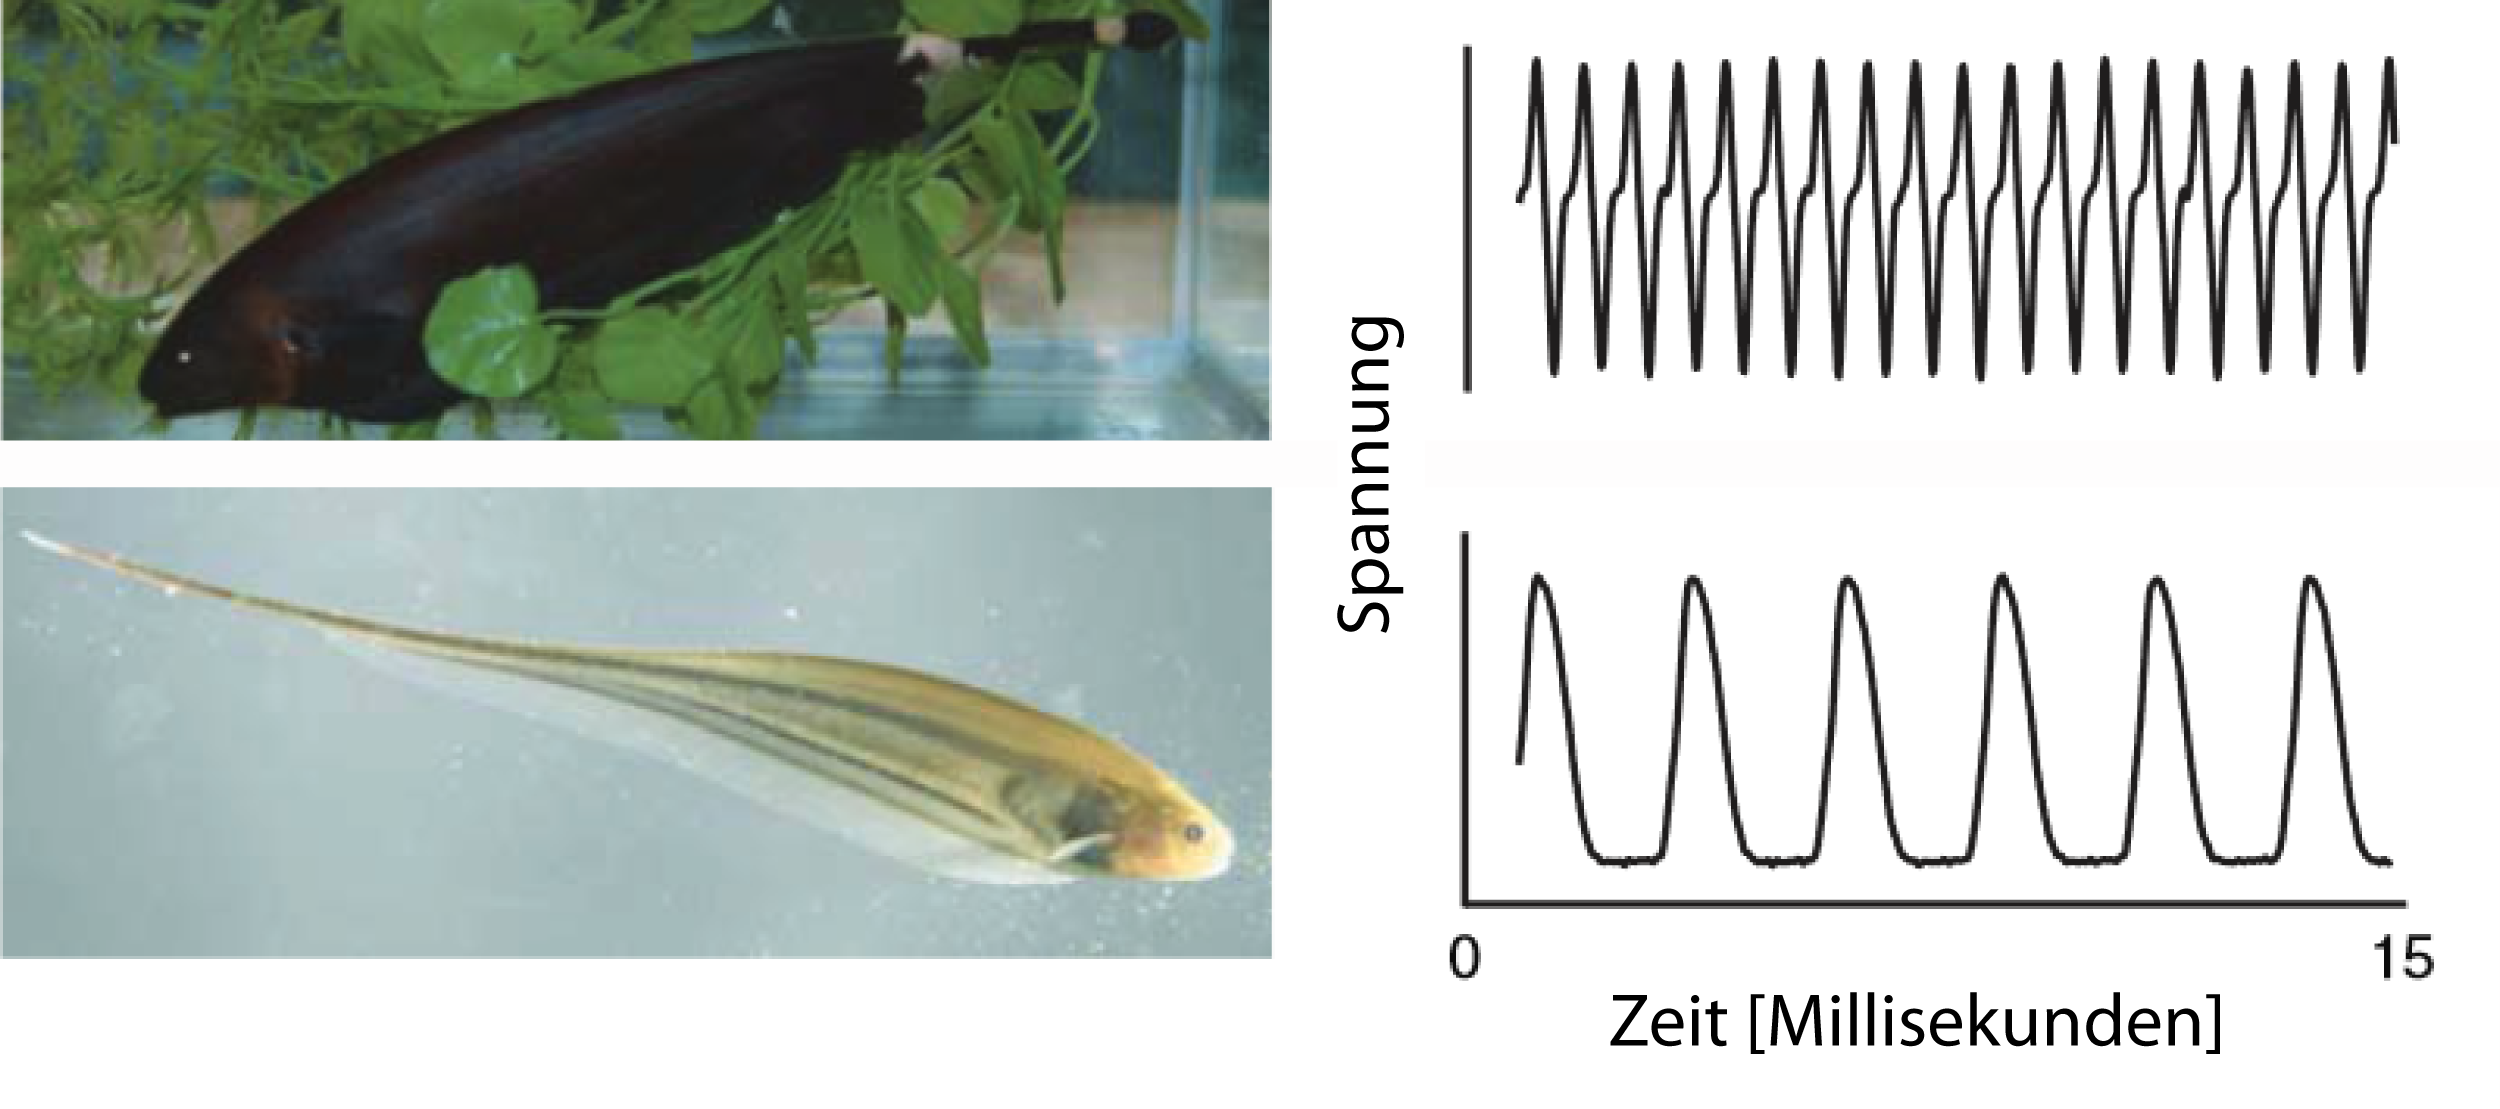
\includegraphics[height=6.5cm]{Abbildungen/waveform}
\caption{\label{fig:waveform} Links: Fotos zweier Arten: Oben ist \emph{Apteronotus albifrons} abgebildet, darunter ein Individuum der Art \emph{Eigenmannia cf. lineata}. Rechts neben den Fotografien sind Signalbeispiele f�r die Wellenformen der beiden Arten zu sehen. Abbildung ver�ndert nach \citet{Fugere2010}}.
\end{figure}

Die Wellenform des EODs ist somit in hohem Ma�e artspezifisch, weshalb sie zusammen mit der EOD Frequenz zur genaueren Bestimmung einer Spezies dienen kann \citep{Fugere2010}. Dar�ber hinaus kann die EOD Frequenz noch weiter Informationen �ber Geschlecht, Alter, Gr��e und Dominanz des Fisches enthalten: So wurde beispielsweise mehrfach eine Korrelation zwischen EOD Frequenz und K�rpergr��e bei \emph{Apteronotus leptorynchus} gezeigt \citep{Dunlap2002, Triefenbach2003}. Au�erdem kann man bei \emph{Apteronotus albifrons} weibliche Individuen anhand ihrer h�heren EOD Frequenz von m�nnlichen Individuen unterscheiden \citep{Dunlap1998}). Die EOD Frequenz wird dabei mittles Steroidhormonen kontrolliert und ist erstaunlich konstan \citep{Meyer1987, Zakon1991, Cuddy2012}. Der EOD generierende Mechanismus wird daher sogar als gleichm��igster bekannter biologischer Oszillator bezeichnet \citep{Moortgat1998}. Jedoch korreliert die EOD Frequenz sehr stark mit der Wassertemperatur, weshalb Schwankungen derselben auch zu Schwankungen der EOD Frequenz f�hren \citep{Enger1968,Dunlap2000}.

N�hern sich zwei oder mehrere schwach elektrische Fische einander an, kommt es zu einer �berschneidung der elektrischen Felder. Da die EODs von Wellenfischen beinahe sinusf�rmig sind, resultiert die �berschneidung zweier EODs in einer Schwebung, im Folgenden Beat genannt. Der Beat ist ein kombiniertes Signal der beiden Einzelsignale, das in seiner Amplitude und Phase oszilliert. Die Beatfrequenz entspricht dabei in etwa der Differenz der beiden EOD Frequenzen \citep{Benda2013}.

Das elektrische Organ, welches die EODs erzeugt, besteht aus mehreren in Reihen und Spalten angeordneten Zellen, sogenannten Elektrozyten \citep{Stoddard2008}. Dabei handelt es sich um scheibenf�rmige, gro�e Zellen, deren Membran zwecks Oberfl�chenvergr��erung gefaltet ist, wodurch es mehr Fl�che f�r spannungsgesteuerte Natrium und Kalium Ionenkan�le gibt \citep{Stoddard2008}.

\begin{figure}[ht]
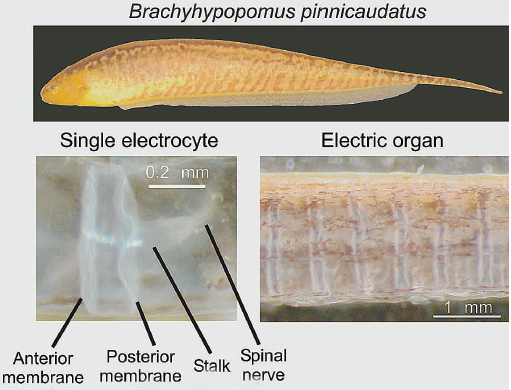
\includegraphics[height=7.5cm]{Abbildungen/ElektrischesOrgan}
\caption{\label{fig:elektrischesorgan} Die Abbildung zeigt am Beispiel des schwach elektrischen Fisches \emph{Brachyopopomus pinnicaudatus} Anatomie und Aussehen einer einzelnen Elektrozyte (links) und des elektrischen Organs (rechts). Der anterioren Membran der Elektrozyte liegt die posteriore Membran gegen�ber. Diese wird durch den Spinalnerv innerviert. Im elektrischen Organ sind die Elektrozyten in Reihen und Spalten angeordnet. Abbildungsquelle: \citet{Stoddard2008}}
\end{figure}

Jede Elektrozyte wird an einer Seite von einem spinalen Motoneuron innerviert (siehe Abb. \ref{fig:elektrischesorgan}). Bei Erregung des Motoneurons kommt es zu einem Aktionspotential an der innervierten (posterioren) Seite der Elektrozyte. Dadurch entsteht an dieser Elektrozytenseite ein Natriumfluss aus dem Extrazellularraum in die Zelle, was zu einer Depolarisation selbiger f�hrt \citep{Stoddard2008}. Da zun�chst nur eine Elekrozytenseite depolarisiert ist, kommt es zu einer ungleichen Ladungsverteilung, wodurch eine Spannung entsteht. Auf den Natrium Influx folgt dann ein Kalium Ausstrom, welcher zur Repolarisierung der Zelle und zum Schlie�en der Natrium Kan�le f�hrt \citep{Stoddard2008}. Die Entladung der einzelnen Elektrozyten wird zentral gesteuert und findet nahezu gleichzeitig statt. Durch die Reihenschaltung der Elektrozyten kommt es dann zu einer Addition der einzelnen Spannungen, wodurch schlie�lich das elektrische Feld um den Fisch herum entsteht \citep{Stoddard2008}. 
Bei den meisten Arten entwickelt sich das elektrische Organ aus Muskelgewebe \citep{Kirschbaum1977, Zakon1999}.Bei der Gattung \emph{Apteronotus} hingegen, besteht das elektrische Organ der adulten Tiere aus modifizierten Axonen von Spinalneuronen \citep{Kirschbaum1983}. Dennoch geht dem neurogenen elektrischen Organ der adult Tiere ein myogenes Organ voraus, welches sich dann nach vollst�ndiger Entwicklung des neurogenen Organs wieder zur�ckentwickelt \citep{Kirschbaum1983}. 

\section{Ampull�re und tuber�se Elektrorezeptoren}

Die Wahrnehmung von elektrischen Signalen erfolgt mittels Elektrorezeptoren \citep{Jorgensen2005}. Sie finden sich nahezu �berall auf der K�rperoberfl�che des Fisches, jedoch mit einer besonders hohen Dichte im Kopfbereich \citep{Zupanc2005}. Gemeinsam mit anderen Hilfszellen formen die Elektrorezeptoren verkapselte Elektrorezeptororane, welche sich in Einst�lpungen der Fischepidermis finden \citep{Zupanc2005}. Die Elektrorezeptororgane kommunizieren dabei mit der K�rperoberfl�che �ber Kan�le, welche mit Schleim oder lose gepackten Epithelzellen gef�llte sind \citep{Zupanc2005} (siehe Abb. \ref{fig:rezeptoren}).

Die in den Rezeptororganen befindlichen Elektrorezeptoren werden von afferenten Nerven innerviert, welche die elektrosensorische Information ans Rhombencephalon, ein ans R�ckenmark angrenzender Gehirnteil, weiterleiten \citep{Zakon1986}.

\begin{figure}[ht]
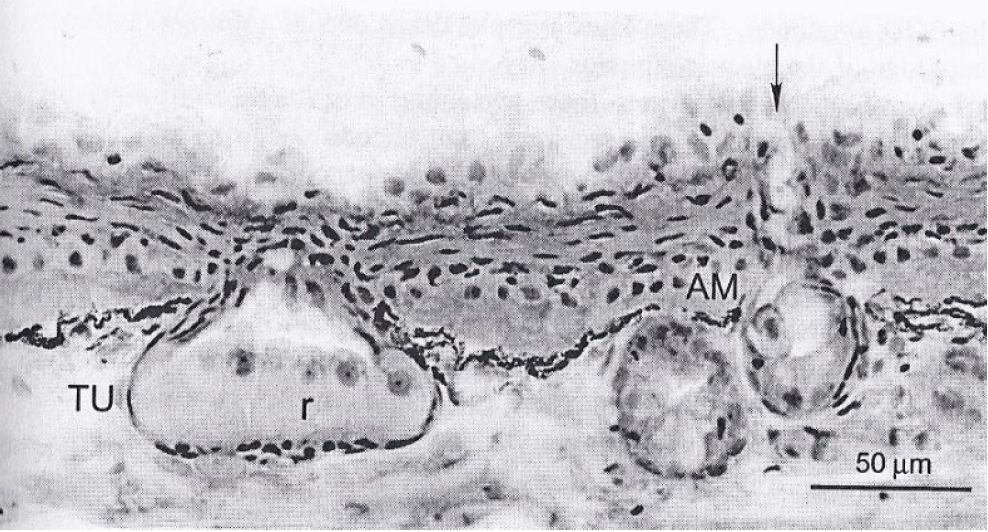
\includegraphics[height=6.5cm]{Abbildungen/Rezeptoren}
\caption{\label{fig:rezeptoren} Zwei Arten von Elektrorezeptororganen in der Haut des Messerfisches \emph{Eigenmannia spec}. Das tuber�se Elektrorezeptororgan (TU), welches links im Bild zu sehen ist, ist nicht direkt mit der Au�enwelt verbunden, sondern durch einen Pfropf epidermaler Zellen verschlossen. Rechts im Bild ist ein ampull�res Elektrorezeptororgan (AM) zu sehen, welches �ber einen schleimgef�llten Kanal direkt mit der Au�enwelt verbunden ist (Bildquelle: \citet{Zupanc2005}).}
\end{figure}

Man unterscheidet grunds�tzlich zwischen zwei Hauptklassen von Elektrorezeptoren:
den tuber�sen und den ampull�ren Elektrorezeptoren.
Die ampull�ren Elektrorezeptoren, wurden bei verschiedensten Fischspezies unter anderem auch bei Haien gefunden und gelten als extrem sensitiv. Fast alle Fische, die nicht zu den \emph{Teleostei} z�hlen ausgenommen der \emph{Myxiniformes} und der \emph{Holostei}, besitzen ampull�re Rezeptoren. Die zu den \emph{Teleostei} z�hlenden \emph{Gynotiformes} und \emph{Mormyriformes} besitzen neben zwei anderen Ordnungen dieser Klasse ebenfalls ampull�re Elektrorezeptoren \citep{Zupanc2005}. Diese ampull�ren Rezeptoren sind im niedrigen Frequenzbereich am empfindlichsten. Hier werden Frequenzen zwischen 0 und 60 Hertz angegeben \citep{Hopkins1976, Nelson1999, Stoddard2008}. Sie detektieren Signale im Microvolt pro Zentimeter Bereich \citep{Stoddard2008}, was eine Wahrnehmung von bioelektrischen Feldern, die jedes lebende Tier umgeben, erm�glicht \citep{Zupanc2005}. 
 
\begin{figure}[ht]
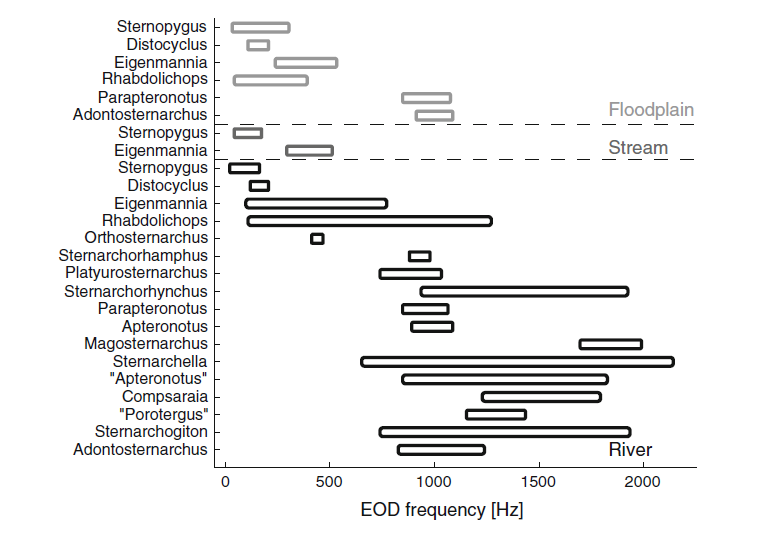
\includegraphics[height=8.5cm]{Abbildungen/EOD_Frequenzen}
\caption{\label{fig:eod_frequenzen} EOD Frequenzbadbreite verschiedener Spezies in verschidenen Habitaten. Die Balken zeigen die Verteilung der EOD Frequenzen der verschiedenen gymnotoiden Gattungen an. In Anf�hrungszeichen gesetzten Namen zeigen an, dass die betroffene Gruppe nicht hinreichend als Genus definiert ist und deshalb als Artengruppe angesehen werden sollte.Abbildungsquelle: \citet{Benda2013}, gezeichnet nach \citet{Crampton2006}}.
\end{figure}
 
Die tuber�sen Elektrorezeptoren hingegen kommen, soweit bislang bekannt, nur bei elektrischen Fischen vor \citep{Stoddard2008}. Sie dienen der aktiven Elektroorung und der Elektrokommunikation mit anderen elektrischen Fischen  \citep{Nelson1999, Stoddard2008}. 
Innerhalb der tuber�sen Rezeptoren unterscheidet man bei gymnotiformen Wellenfischen zwischen zwei Unterpopulationen: Den P-Units und  den T-Units \citep{Scheich1973, Heiligenberg1977, Zupanc2005}.
Die T-Units sind Rezeptoren, die eins zu eins auf jeden EOD Zyklus mit einem Aktionspotenzial antworten. Damit spiegeln sie den zeitlichen Ablauf der EODs wider \citep{Zupanc2005}.
Die zweite Kategorie, die sogenannten P-Units, hingegen feuern probabilistisch, sprich mit einer Zufallskomponente.  Ihre Antwortwahrscheinlichkeit auf ein EOD h�ngt dabei von der EOD Amplitude ab \citep{Zupanc2005}.
Die tuber�sen Rezeptoren sind f�r Signale mit Frequenzen im Bereich der fischeigenen EOD Frequenz am empfindlichsten \citep{Hopkins1976, Zupanc2005}. So kam 
\citet{Hopkins1976} bei seinen Untersuchungen der Elektrorezeptoren zu dem Ergebnis, dass das Tuning der tuber�sen Elektrorezeptoren auf die fischeigene EOD Frequenz abgestimmt ist, was bei \emph{Apteronotus albifrons} einem  EOD Frequenzbereich von 800 bis 1200 Hertz entpspricht. 
Das speziesspezifische Tuning der tuber�sen Elektrorezeptoren sieht \citet{Hopkins1976} dabei als wichtige Vorraussetzung f�r eine ungest�rte Kommunikation und Elektroortung bei gymnotoiden Fischen. Da die Bandbreite von Frequenzen, die eine P-Unit Antwort ausl�sen, durch das Rezeptortuning begrenzt ist, ist die Wahrnehmung anderer Arten, die andere Frequenzbandbreiten nutzen stark begrenzt. Man ging daher von Spezies spezifischen Kommunikationskan�len aus, innerhalb welcher einzelne Spezies Signale abgeben und wahrnehmen k�nnen. Abbildung \ref{fig:eod_frequenzen} zeigt hierbei die verschiedenen Frequenzbereiche verschiedener Gattungen in unterschiedlichen Habitaten.
Dennoch �berlappen sich bei vielen sympatrisch lebenden Spezies die Frequenzbereiche \citep{Kramer1981}, was g�nzlich private Kommunikationskan�le ausschlie�t. Au�erdem zeigen einige Forschungen, dass f�r die Elektrokommunikation ein breiteres Tuning der Elektrorezeptoren n�tig ist. So k�nnen bei der Kommunikation mit einem Partner von anderen Geschlecht wegen der gro�en EOD Frequenzdifferenz Beatfrequenzen bis zu 400 Hertz entstehen \citep{Benda2013}. Dar�ber hinaus kommt es bei Kommunikationssignalen wie bei den sogenannten 'Chirps' zu kurzen Frequenzerh�hungen um mehrere Hertz \citep{Hagedorn1985}. Daraus l�sst sich schlie�en, dass P-Units offenbar ein breiteres Tuning brauchen als beispielsweise von \citet{Hopkins1976} angenommen, um alle relevanten Signale aufzunehmen. 


\section{Ziel der Arbeit}

\infobox{Harmonische}{Es gelten folgende Bezeichnungen: Die Grundschwingung der Frequenz f wird als 1. Harmonische bezeichnet, eine Schwingung der doppelten Frequenz (2f) als 2. Harmonische. Allgemein ist die Schwingung mit der n-fachen Frequenz der Grundfrequenz (nf) die n. Harmonische.}
Wie von Fourier beschrieben, kann jedes periodische Signal in mehrere Sinusschwingungen mit jeweils n-facher Frequenz der Grundschwingung aufgedr�selt werden. 
Die Frequenz der Grundschwingung von \emph{Eigenmannia virescens} liegt bei etwa 250 bis 500 Hertz \citep{Hopkins1976} (siehe Abb. \ref{fig:powerspektrum}). Die Frequenz der zweiten Harmonischen liegt demnach im Bereich von 500 bis 1000 Hertz und �berschneidet sich mit dem Frequenzbereich von \emph{Apteronotus albifrons}. Die zweite Harmonische sollte f�r \emph{Apteronotus albifrons} also wahrnehmbar sein. 
Noch unver�ffentlichte elektrophysiologische Studien weisen au�erdem darauf hin, dass die P-Units von \emph{Apteronotus albifrons} auch auf Frequenzen im Bereich der Grundschwingung von \emph{Eigenmannia} antworten. 
\begin{figure}[ht]
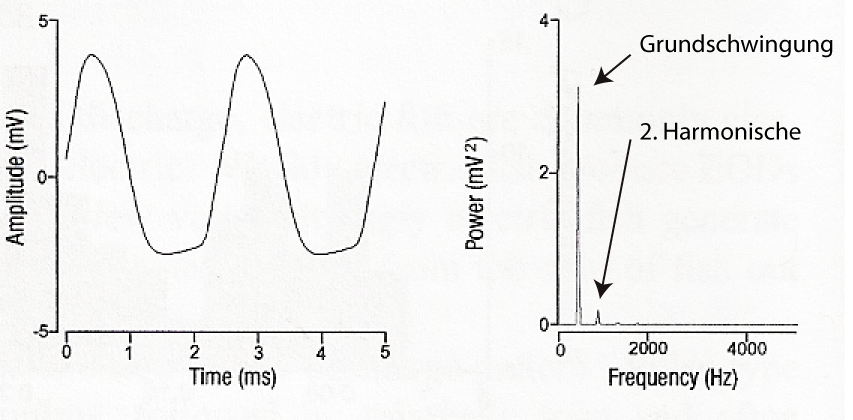
\includegraphics[height=5.5cm]{Abbildungen/powerspektrum}
\caption{\label{fig:powerspektrum} Links: EOD von \emph{Eigenmannia spec.} mit der arttypischen Wellenform. Rechts: Die Spektrale Zusammensetzung des Signals in Form eines Fourierspektrums. Auf der X-Achse sind die Frequenzen der einzelnen Schwingungen, aus welchen sich das EOD zusammensetzt aufgetragen. Auf der Y-Achse ist die Amplitude der Schwingung aufgetragen. Der erste Spike im Frequenzbereich 400 Hertz stellt die Grundschwingung dar. Der zweite deutlich kleinere Spike ist die zweite Harmonische. Abbildung ver�ndert nach \citet{Zupanc2005}}.
\end{figure}

Ziel dieser Arbeit war es daher zu �berpr�fen, ob \emph{Apteronotus albifrons} dazu in der Lage ist Frequenzen im Bereich einer Eigenmannia Grundschwingung wahrzunehmen.
Dies sollte mittels operanter Konditionierung der Versuchstiere in einem Verhaltensversuch getestet werden.


\chapter{Material und Methoden}

\section{Versuchstiere}

F�r diese Arbeit wurde mit vier Messerfischen der Art \emph{Apteronotus albifrons} gearbeitet, welche von dem Tiergro�h�ndler Aquarium Glaser, Rodgau stammten. Zwei der Versuchstiere (Fisch 1 und Fisch 2) waren Jungtiere, welche wenige Tage vor Versuchsbeginn eingetroffen waren.  Bei den beiden anderen \emph{Apteronoti} (Fisch 3 und Fisch 4) handelte es sich um adulte Tiere, welche bereits in den Jahren 2013 (Fisch 3) und 2014 (Fisch 4) bezogen worden waren. Die vier Versuchstiere waren naiv und hatten zuvor an keinem anderen Experiment teilgenommen. 
Die Jungtiere unterschieden sich mit einer K�rperl�nge von etwa neun Zentimetern deutlich von den adulten Tieren, welche eine K�rperl�nge von etwa 18 Zentimetern ma�en.\\
Zu einem sp�teren Zeitpunkt wurden noch zwei weitere adulte Tiere, ebenfalls der Art \emph{Apteronotus albifrons} (Fisch 5 und Fisch 6), in den Versuch einbezogen. Diese hatten bereits neun Monate zuvor an einem �hnlichen Experiment teilgenommen und kannten den Versuchsablauf. Diese Fische waren in den Jahren 2013 (Fisch 5) und 2012 (Fisch 6) bezogen worden.
Die Versuchstiere wurden au�erhalb der Versuche in Aquarien mit den Ma�en 81cm x 50cm x 50cm gehalten. Diese waren durch Gitter in einzelne etwa 30cm x 50cm x 50cm gro�e Kompartimente unterteilt, was eine elektrische Kommunikation zwischen den Fischen erm�glichte, k�rperliche Auseinandersetzungen aber unterband. Fisch 1 wurde isoliert in einem Tank gehalten, welcher �ber die gleichen Ma�e wie die einzelnen Kompartimente verf�gte.
Da die Versuchstiere nachtaktiv sind, wurde der Zw�lf-Stunden-hell-dunkel-Rhythmus so eingestellt, dass ab zw�lf Uhr drei�ig das Licht ausgeschaltet wurde. Die aktive Phase der Fische war dann gegen Nachmittag.
Die Wassertemperaturen in den Aquarien wurden zwischen 25 Grad Celsius und 27,5 Grad Celsius gehalten.

\section{Versuchsbecken}

Das Versuchsbecken mit den Ma�en 100cm x 50cm x 40cm ist in Abbildung \ref{fig:setup1} im Grundriss zu sehen. Eine Kunststoffplatte unterteilte das Becken in Hauptbecken und Startbox. �ber ein in die Kunststoffplatte eingelassenes Tor konnte der Zugang der Startbox ins Hauptbecken ge�ffnet und geschlossen werden.
Im Hauptbecken wurde an jeder L�ngsseite auf gleicher H�he je eine Stimuluselektrode am Beckenrand angebracht. In der Startbox befand sich ebenfalls an der L�ngsseite des Versuchsbeckens jeweils eine Ableitelektrode, welche die EOD des Fisches und die von den Stimuluselektroden abgegebenen Stimuli ma�. Au�erdem wurde eine Erdungselektrode in die Startbox gegeben, um elektrisches St�rrauschen im 50-Hertz-Bereich zu reduzieren.

Abbildung \ref{fig:setup2} (a) zeigt den Versuchsaufbau in der Seitenansicht. Das Versuchsbecken war von au�en mit dunkelblauen M�lls�cken abgeklebt, um eine Orientierung des Versuchstieres an Markierungspunkten au�erhalb des Beckens zu vermeiden. Zus�tzlich wurde dadurch der Lichteinfall von St�rlichtquellen wie dem Computerbildschirm ins Innere des Versuchsbeckens minimiert. Mittig �ber dem Versuchsbecken war eine Infrarotkamera (Guppy F044B NIR Allied Vision Technologies GmbH) angebracht. Zwischen den acht Styroporbl�cken, auf welchen das Versuchsbecken stand, waren an jeder L�ngsseite vier Infrarotlampen positioniert. Die Infrarotlampen (Abus IR Strahler, Wellenl�nge 840 Nanometer) bestrahlten den Beckenboden von unten und wurden durch eine Kabelreihe geerdet.Um eine Reflektion und Streuung des Infrarotlichts zu vermeiden, wurde eine Transparenzfolie auf den Beckenboden geklebt. Zur Erh�hung der Helligkeit der Videoaufnahmen wurde au�erdem der Tisch, auf dem der Versuchsaufbau stand,mit wei�em Papier beklebt.
Au�erhalb der Versuchszeiten wurden ein Heizstab (Eheim J�ger 3614 Aquarium Heater) und ein Filter (Eheim) in das Versuchsbecken gegeben. 
Die Wassertemperaturen des Versuchsbeckens wurden konstant auf 27 Grad Celsius (+- 0,6) gehalten. Die Wassertemperatur wurde vor jedem Versuch mit einem Thermometer von Extech Instruments (EC400: ExStik� Conductivity/TDS/Salinity Meter) erfasst. Alle 14 Tage wurde ein vollst�ndiger Wasserwechsel durchgef�hrt.

\begin{figure}[ht]
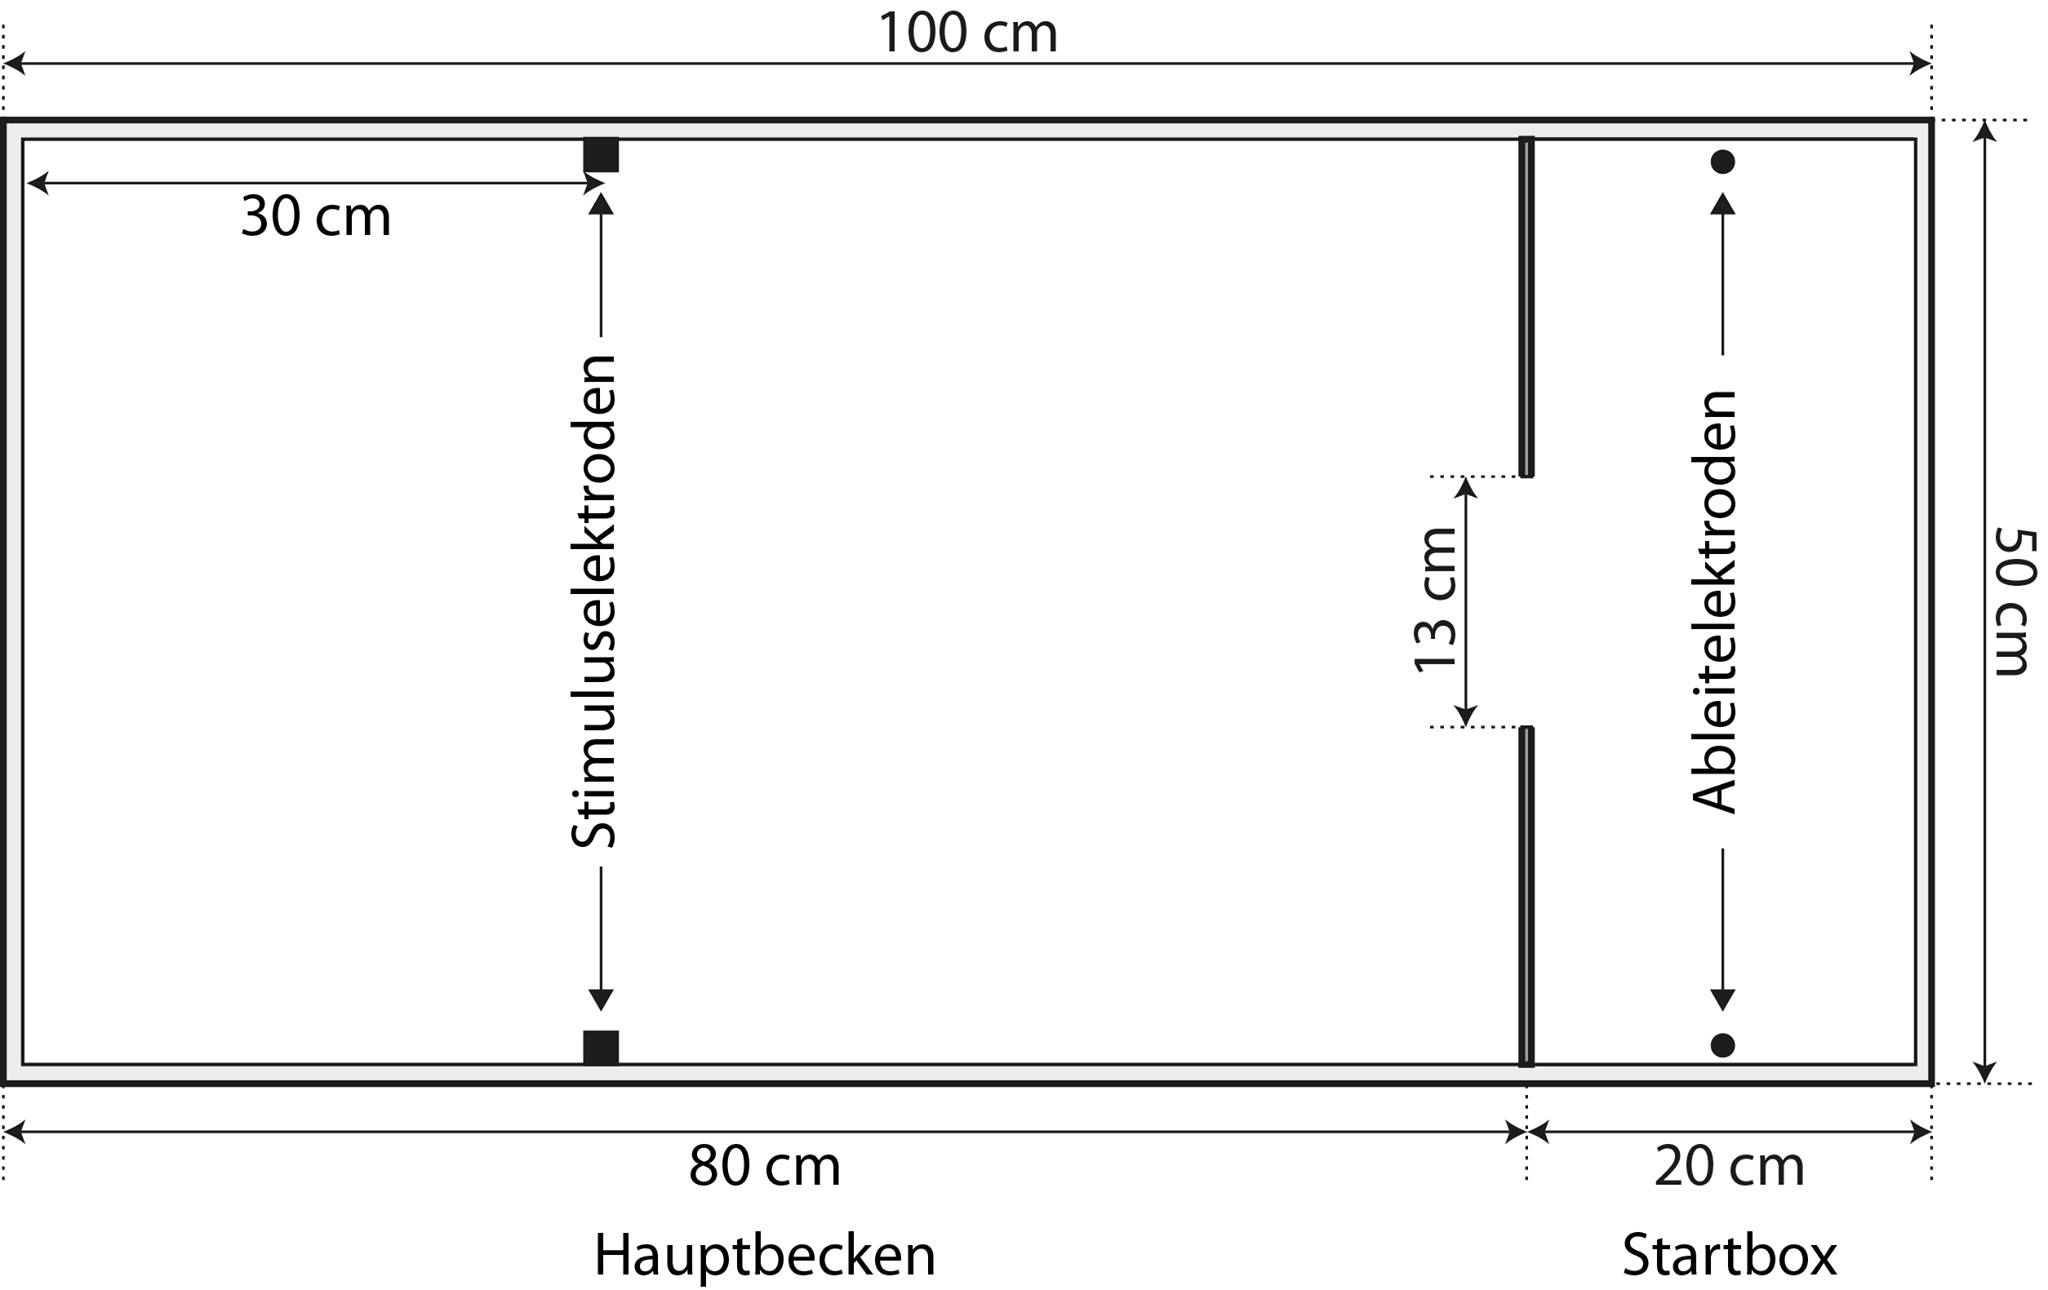
\includegraphics[height=6.5cm]{Abbildungen/Setup1}
\caption{\label{fig:setup1}Versuchsbecken von oben. Links: Hauptbecken mit je einer Stimuluselektrode an den L�ngsseiten, rechts: Startbox mit Ableitelektroden}
\end{figure}

\begin{figure}
\subfigure[Versuchsaufbau von oben nach unten: Infrarotkamera, Versuchsbecken, Styroporplatten mit Infrarotlampen in den Zwischenr�umen.]{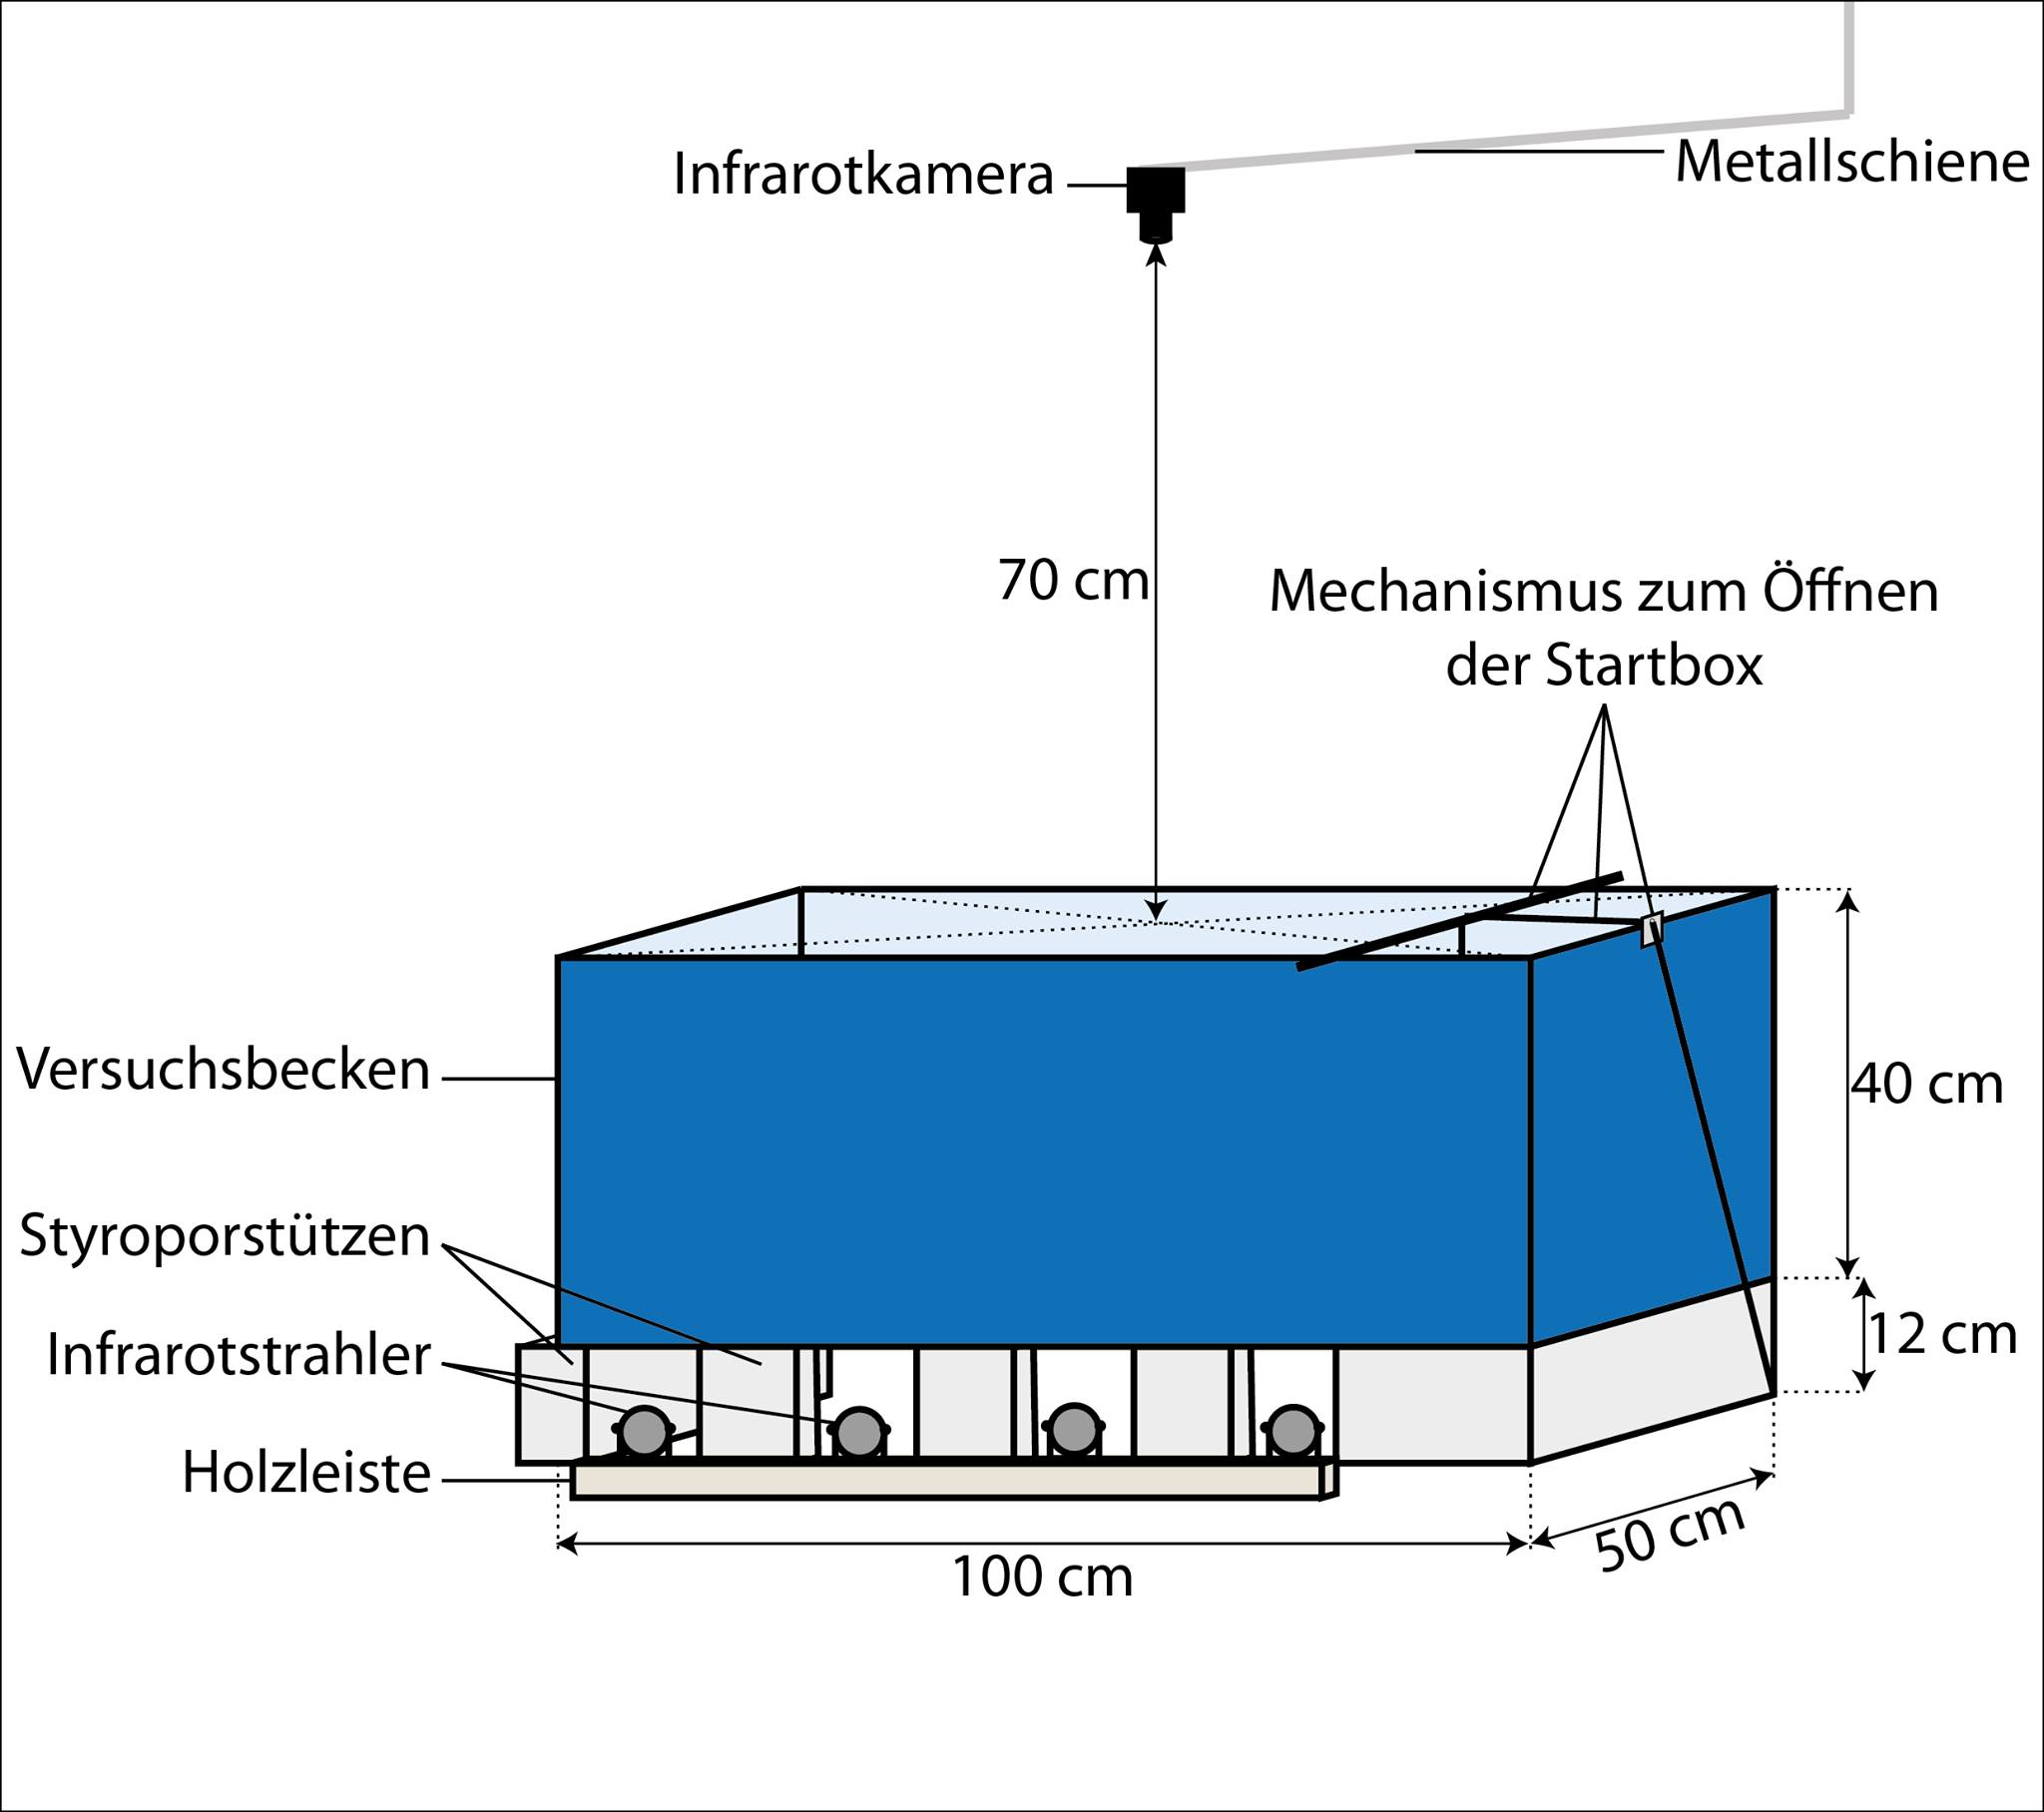
\includegraphics[height=8.5cm]{Abbildungen/Setup2}}\hfill
\subfigure[Stimuluselektrode]{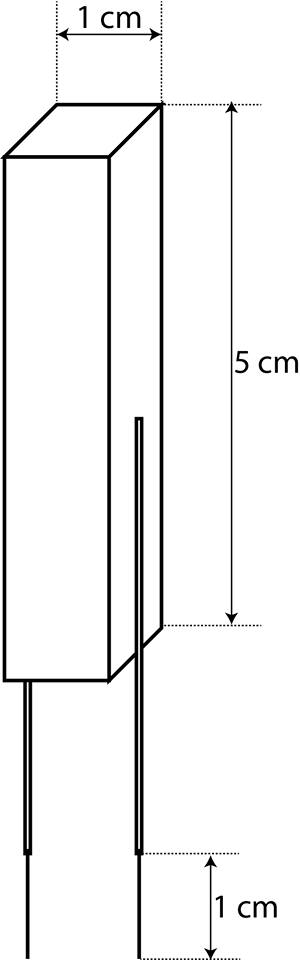
\includegraphics[height=8.5cm]{Abbildungen/Stimuluselektrode}}
\caption{\label{fig:setup2}Versuchsaufbau}
\end{figure}

\section{Die Elektroden}

\subsection{Stimuluselektroden}
Die in Abbildung \ref{fig:setup2} (b) gezeigten Stimuluselektroden gaben die elektrischen Stimuli ins Versuchsbecken ab. Die Enden der Stimuluselektroden waren nicht isoliert, so dass das reine Silberkabel in Kontakt mit dem Wasser stand.
Die computergenerierten Stimuli wurden vom Computer (Fujitsu, Esprimo P710 E85+) an den Analog-Digitalwandler (NI BNC 2090) weitergegeben. Dieser leitete das elektrische Signal dann �ber einen Verst�rker (DPA 2FS npi) an die Stimuluselektroden weiter, welche den Reiz ins Wasser abgaben.
Um zu ermitteln, wie die elektrischen Felder der Stimuluselektroden im Becken aussahen, wurde das elektrische Feld beider Stimuluselektroden vermessen.
Abbildung \ref{fig:heatmaps} zeigt dabei die auf eins normierte Stimulusintensit�t an jeder Position im Versuchsbecken f�r Elektrode 1 (Abb. \ref{fig:heatmaps} (a)) und Elektrode 2 (Abb. \ref{fig:heatmaps} (b)). Die Stimuli wurden im Versuchsbecken im Abstand von f�nf Zentimetern jeweils zehn Sekunden lang gemessen. Anschlie�end wurde aus den so gewonnenen Daten f�r jede gemessene Beckenposition die mittlere Intensit�t ermittelt. 


\begin{figure}
\subfigure[Elektrisches Feld von Elektrode 1]{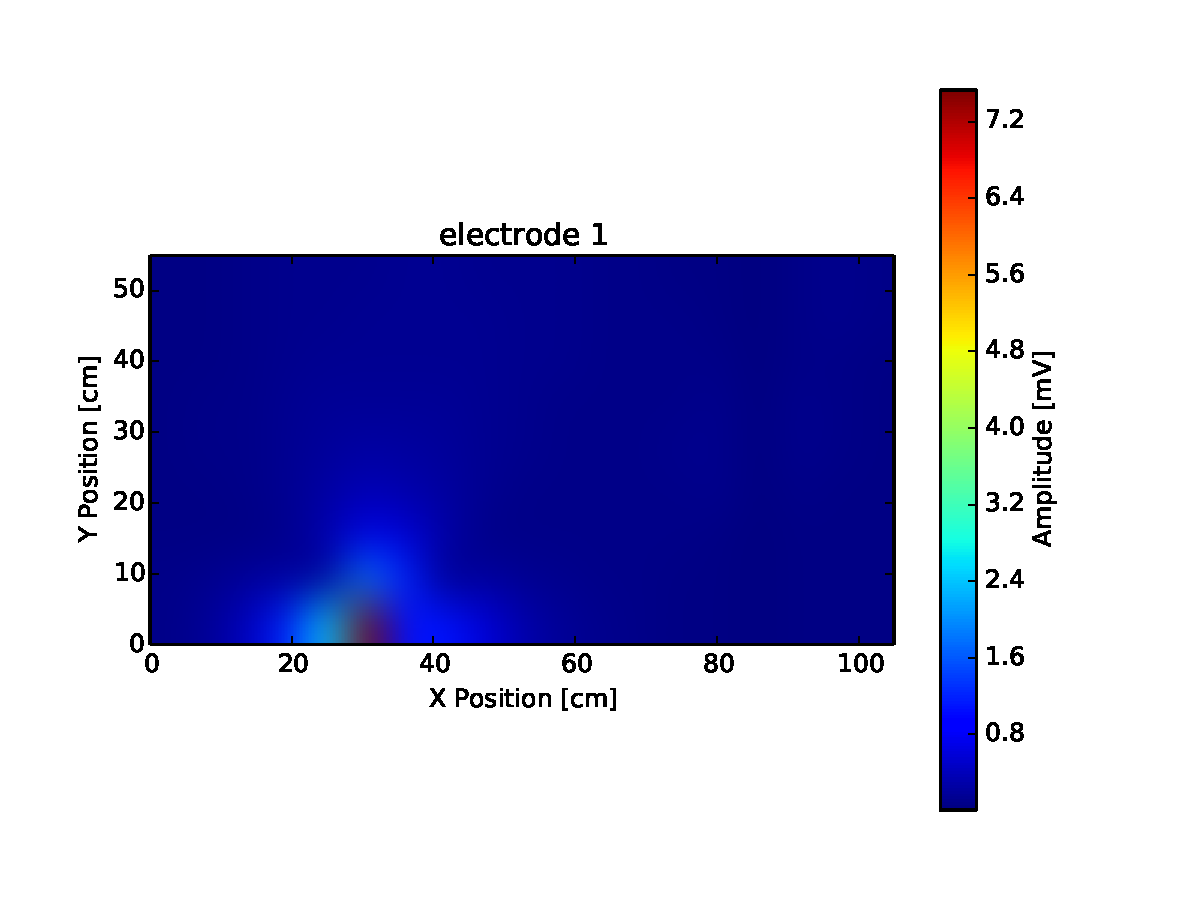
\includegraphics[height=7cm]{Abbildungen/Heatmap_E1}}\hfill
\subfigure[Elektrisches Feld von Elektrode 2]{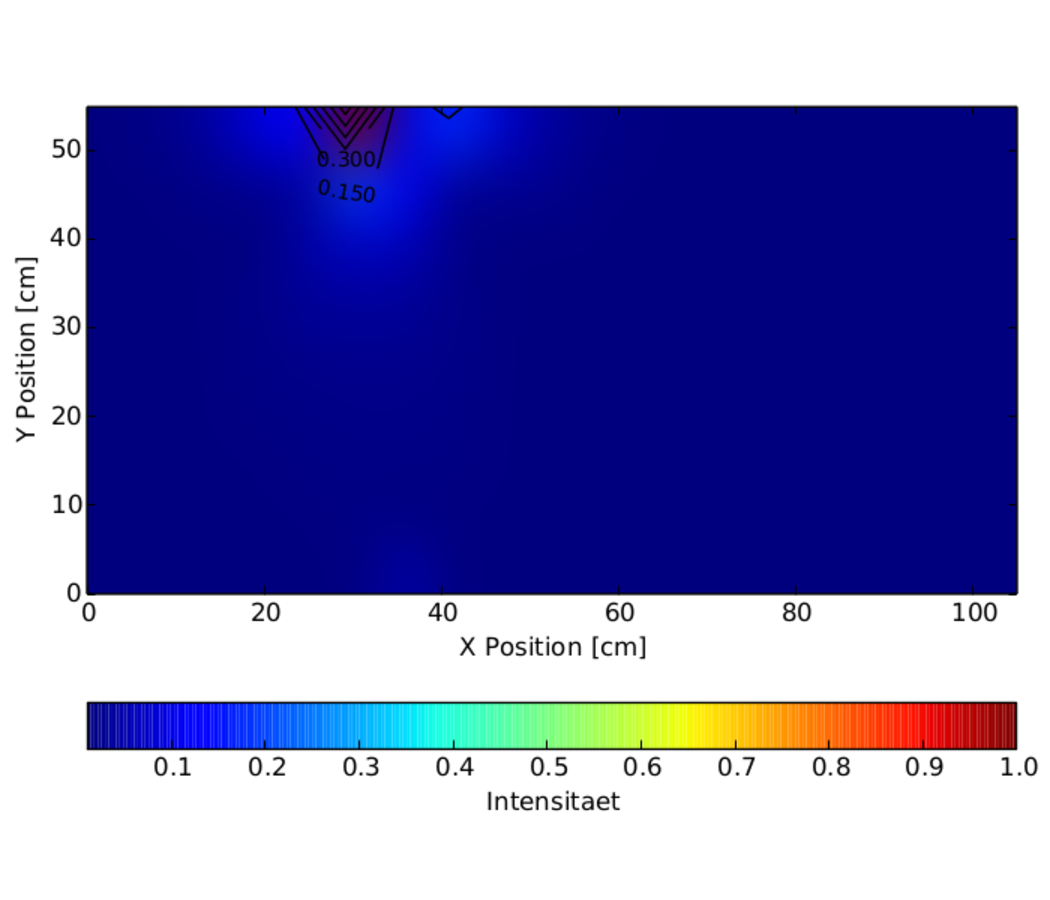
\includegraphics[height=7cm]{Abbildungen/Heatmap_E2}}
\caption{\label{fig:heatmaps}Normierte Intensit�ten von Elektrode 1 und Elektrode 2 f�r jede Position im Becken. Einstellungen im Messprogramm  "Relacs - Dual Field Amplitudes": Amplitude: 1 Volt, Frequenz: 1000 Hz}
\end{figure}


Um sicherzustellen, dass die abgegebenen Stimuli zumindest an einer Position im Becken eine gleiche Intensit�t hatten, wurden sie folgenderma�en kalibriert: In einer mittigen Position zwischen den beiden Stimuluselektroden wurde jeweils die Amplitude von Elektrode 1 und von Elektrode 2 ermittelt. Anschlie�end wurden die Amplituden der beiden Stimuluselektroden durch Ausprobieren verschieder Skalierungsfaktoren so eingestellt, dass sie bis auf zwei Nachkommastellen �bereinstimmten (siehe Tabellen \ref{amplitude1} und \ref{amplitude2}). Dadurch ergaben sich f�r die Elektroden folgende Skalierungsfaktoren: Das Signal von Elektrode 1 wurde um den Faktor 0,7 skaliert, das von Elektrode 2 um den Faktor 2. Zus�tzlich wurden in den Versuchen die Amplituden zuf�llig um +- 20 Prozent skaliert.


\begin{table} [h] 
	\centering
	\caption{Messung der Amplitude von Elektrode 1}
	\vspace{0,2cm}
	\begin{tabular}{lccc} %eigentliche Tabelle 
		{\textbf{Elektrode 1 Scale: 0,7}}  \\
		\toprule % d�nne Linie 
		& Messung 1 & Messung 2  & Messung3 \\
		 Minimum [mV]:& -0,17624  & -0,17136 & -0,17075 \\
		 Maximum [mV]:& 0,10605  & 0,10605 & 0,11673 \\
		 Differenz [mV]: & 0,28229 & 0,277410 & 0,28748 \\
		\bottomrule % bi�chen dickere Linie unten
		\vspace{0,2cm}
		{Mittelwert [mV]: 0.28239} \\
	\end{tabular}\\
	\label{amplitude1}
\end{table}
	
	
\begin{table} [h] 
	\centering
	\caption{Messung der Amplitude Elektrode 2}
	\vspace{0,2cm}	
	\begin{tabular}{lccc} %eigentliche Tabelle 
		{\textbf{Elektrode 2 Scale: 2,0}} \\
		\toprule % d�nne Linie 
		& Messung 1 & Messung 2  & Messung3 \\
		 Minimum [mV]:& -0.16007  & -0.1622 & -0.15122 \\
		 Maximum [mV]:& 0.11673  & 0.130 & 0.13291 \\
		 Differenz [mV]: & 0.2768 & 0.2922 & 0.28413 \\
		\bottomrule % bi�chen dickere Linie unten
		
		{Mittelwert [mV]: 0.28438} \\
	\end{tabular}
	\label{amplitude2}
\end{table}

\subsection{Ableitelektroden}
Die Ableitelektroden befanden sich in der Startbox und hatten die Funktion, die EOD des Versuchstieres zu messen. Hierbei handelte es sich um Kupferelektroden, welche separat zu den Stimuluselektroden mit einem zweiten Verst�rker verbunden waren. Das Signal wurde anschlie�end �ber den Analog-Digitalwandler (NI BNC 2090) digitalisiert und an den Computer weitergegeben.

\section{Aufnahmeprogramme}
Zur Aufnahme der Daten wurde das Programm "Relacs Version 0.9.8" verwendet. Bei der Intensit�ten von Elektrode 1 und 2 (siehe Abbildung \ref{fig:heatmap1} und \ref{fig:heatmap2}) wurde das Repro "Dual Field Amplitudes" verwendet. Bei allen anderen Messungen wurde mit dem Repro "Dual Beat" gearbeitet.

\chapter{Durchf�hrung}
Alle Versuche wurden nachmittags im Dunkeln durchgef�hrt. Der Grundablauf war dabei folgender: Zun�chst wurden Wassertemperatur, Wasserstand und Leitf�higkeit im Versuchsbecken gemessen und notiert. Wichen diese stark von den festgesetzten Werten ab, so wurden Wasserstand, Temperatur und Leitf�higkeit im Versuchsbecken durch Wasserwechsel angepasst. Die festgesetzten Werte waren folgende Wasserstand = 14 (+- 0,2) Zentimeter, Leitf�higkeit = 300 (+- 20) Microsiemens pro Zentimerter, Temperatur 27 (+- 0,6) Grad Celsius. Anschlie�end wurde das Versuchstier mit einem Kescher in die Startbox gesetzt. Der Zugang zur Hauptbox war zu diesem Zeitpunkt geschlossen. W�hrend sich das Tier in der Startbox befand, wurde die EOD Frequenz des Fisches gemessen und anschlie�end die Startbox ge�ffnet. Nach Beenden der Aufgabe wurde das Tier dann vorsichtig mit einem K�scher zur�ck in die Startbox gef�hrt. Anschlie�end wurde der n�chste Durchlauf gestartet. Jedes Versuchstier hatte pro Versuchstag zehn Versuchsdurchl�ufe.

\section{Hauptversuch}

\subsection{Einfaches und eigenmanniaartiges Signal}

Ziel des Versuches war es herauszufinden, ob die Versuchstiere den einfachen Stimulus von einem eigenmanniaartigen Stimulus (siehe Abb. \ref{fig:frequenzen} unterscheiden k�nnen.

\textbf{Einfaches Signal:}
Bei dem einfachen Signal handelte es sich um ein elektrisches Signal, welches aus einer einzelnen Frequenz bestand. Diese Frequenz unterschied sich von der EOD Frequenz des Versuchstiers um einen f�r jeden Fisch individuell festgelegten Wert im Bereich von - 100 Hertz bis + 100 Hertz. Bei einer �berlappung des einfachen Signals mit der EOD Frequenz des Fisches entstand im Versuchsbecken eine Schwebung, welche der Frequenzdifferenz der beiden Signale entsprach. Diese Schwebung wird im Folgenden Beat genannt. Jedes Versuchstier wurde auf einen individuellen Beat trainiert. Da die EOD Frequenz der Versuchstiere in den Versuchsdurchl�ufen schwankte, wurde auch die Frequenz des einfachen Signals vor jedem Versuchsdurchlauf so moduliert, dass der aus den beiden Frequenzen resultierende Beat konstant war . Auf welchen Beat jedes Versuchstier trainiert wurde, kann in Tabelle \ref{beats}) nachgelesen werden.

\textbf{Eigenmanniaartiges Signal:} 
Das eigenmanniaartige Signal setzte sich im Gegensatz zum einfachen Signal aus zwei verschiedenen Frequenzen zusammen. Zu der Frequenz des einfachen Signals wurde noch die zugeh�rige Basisfrequenz abgegeben. Die Basisfrequenz entspricht genau der halben Frequenz des einfachen Signals (siehe Abb. \ref{fig:frequenzen}). Dadurch entstand ein Signal, welches dem der Gattung \emph{Eigenmannia} sehr �hnlich ist. Im Versuchsbecken entstand dann zum einen der gleiche Beat wie beim einfachen Signal. Zus�tzlich dazu kam es aber auch zu einem sehr hohen Beat, welcher durch die �berlappung der Fisch EOD mit der Basisfrequenz entstand.   

Die Generierung der Stimuli erfolgte folgenderma�en: Vor jedem Versuchsdurchlauf wurde die EOD Frequenz des Fisches gemessen. Anschlie�end wurde dann das Signal passend dazu mit der entsprechenden Frequenzdifferenz am Computer generiert und von den Stimuluselektroden abgegeben. 
Welcher S+ Stimulus (belohnter Reiz) und welcher S- Stimulus (unbelohnter Reiz) f�r die Versuchstiere festgelegt wurde, kann in folgender Tabelle nachgelesen werden: Tabelle \ref{beats}.


\begin{table} [h] 
	\centering
	\caption{ Die Tabelle zeigt die S+ und S- Stimuli, auf welche die einzelnen Versuchstiere trainiert wurden. Das Fischsymbol (\PHtunny)  steht f�r ein eigenmanniaartiges Signal. Steht nichts hinter der angegebenen Beatfrequenz, handelt es sich um einen einfachen Stimulus.}
	\vspace{0,2cm}	
	\begin{tabular}{llll} %eigentliche Tabelle 
		\toprule % d�nne Linie 
		& S+ & S-\\
		 Fisch 1 (2015albi02):& +40 Hz & +40 Hz \PHtunny \\
		 Fisch 2 (2015albi01):& +60 Hz & +60 Hz \PHtunny \\
		 Fisch 3 (2014albi08):& - 60 Hz \PHtunny & - 60 Hz \\
		 Fisch 4 (2013albi14):& - 40 Hz \PHtunny & - 40 Hz \\
		 Fisch 5 (2013albi09):& +100 Hz & +100 Hz \PHtunny\\
		 Fisch 6 (2012albi01):& +40 Hz & +40 Hz \PHtunny \\
		\bottomrule % bi�chen dickere Linie unten
	\end{tabular}
	\label{beats}
\end{table}


\begin{figure}[ht]
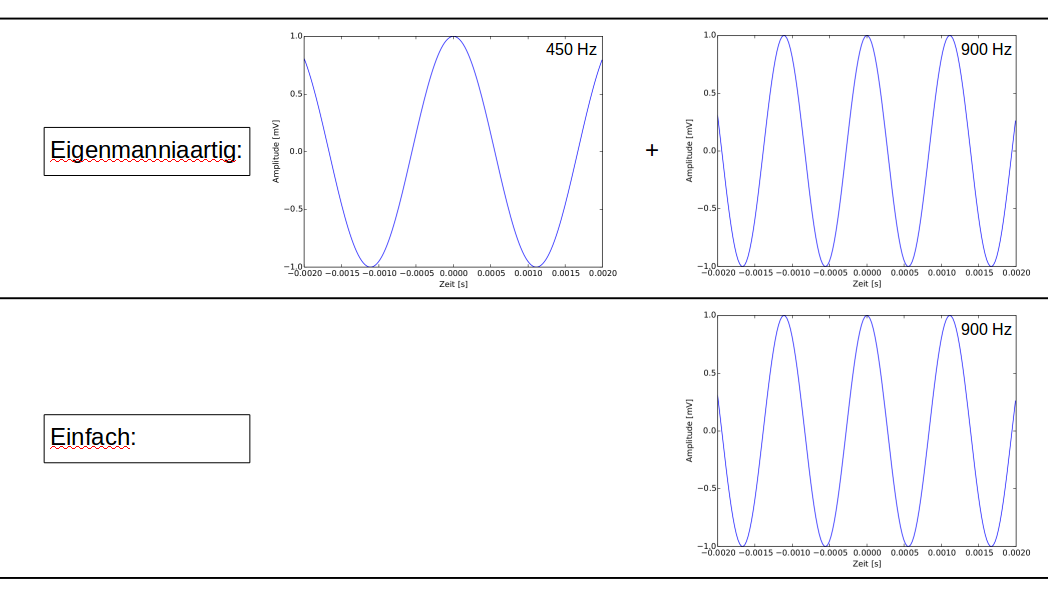
\includegraphics[height=6.5cm]{Abbildungen/frequenzen}\\
\caption{\label{fig:frequenzen}Gegen�berstellung des eigenmanniaartigen und des einfachen Stimulus}
\end{figure}

\subsection{Versuchsablauf}

Der Versuch lief folgenderma�en ab: Zun�chst wurde die Videoaufnahme mittels der Inrarotkamera gestartet. Anschlie�end wurde mit Relacs die EOD Frequenz des Fisches gemessen. Aufgundlage dessen wurde dann der S+ und S- Stimulus generiert und von den Stimuluslektroden abgegeben. Sobald das Signal aktiv war, wurde die Startbox ge�ffnet.

W�hlte der Fisch innerhalb der 60 Sekunden, in welchen die Stimuli aktiv waren, die richtige Elektrode aus, wurde zun�chst die Videoaufnahme gestoppt und anschlie�end die Belohnung mit der Pipette verabreicht. Erst nach der Belohnung wurde der Stimulus mittels Relacs beendet. 
Im Falle einer falschen Elektrodenwahl des Fisches wurden das Videotracking und der Stimulus beendet. Anschlie�end wurde das Versuchstier ohne Belohnung in die Startbox zur�ckgef�hrt. 
Sollte der Fisch innerhalb der 60 Sekunden Aktivit�tsspanne der Stimuluselektroden sich f�r keine der beiden Elektroden entschieden haben, wurde die Videoaufnahme nach Ablauf der 60 Sekunden beendet und der Fisch ohne Belohnung in die Startbox zur�ckgef�hrt. 
Pro Versuchstag hatte jeder Fisch zehn Versuchsdurchl�ufe. Alle Durchl�ufe wurden nachmittags und im Dunkeln durchgef�hrt. Nach jedem Durchlauf wurden die Leitf�higkeit und Temperatur des Wassers gemessen und notiert. Die Wassertemperatur wurde dabei konstant auf 27 Grad Celsius (+- 0,6 Grad Celsius) gehalten. Die Leitf�higkeit des Wassers betrug 300 Microsiemens pro Zentimeter (+- 25 Microsiemens/Zentimeter)

Der Versuchsdurchf�hrende sa� w�hrend des Versuchs mit dem R�cken zum Versuchsbecken und beobachtete mit Hilfe der Videoaufnahmen die Vorg�nge im Versuchsbecken auf dem Computerbildschirm. Erst nach einer Entscheidung und Beendigung der Videoaufnahme stand die Versuchsperson auf, um das Versuchstier zu belohnen.
Eine Elektrode galt als ausgew�hlt, wenn das Versuchstier mindestens drei Sekunden an der Elektrode mit einem geringeren Abstand als f�nf Zentimetern verweilte und zur Elektrode hin orientiert war.

\subsection{Ver�nderung der Amplitude}
Um zu testen, ob eine ver�nderte Stimulusamplitude das Verhalten der Versuchstiere beeinflusst, wurde die Amplitude von einem mV auf zwei Millivolt verdoppelt. Der Versuch wurde sonst genauso wie zuvor durchgef�hrt. 

\subsection{Umkehrung von S+ und S- Stimulus}
S+ und S- Stimulus von einem der Versuchstiere (Fisch 2) wurden vertauscht. Der Versuch lief ansonsten genauso ab wie zuvor.

\section{Vorversuche}
Zur schrittweisen Vorbereitung auf den Hauptversuch durchliefen die Versuchstiere Fisch 1 bis Fisch 4 folgende Vorversuche:

\subsection{Eingew�hnung}
Ziel des Versuchs war die Gew�hnung der Tiere an das Versuchsbecken und an die F�tterung an den Stimuluselektroden. 
Die Aufgabe des Versuchstieres bestand darin, die Startbox aus Eigeninitative zu verlassen und die an den Elektroden platzierten M�ckenlarven zu finden und zu fressen. Mittels M�nzwurf wurde vor jedem Durchlauf entschieden, an welcher Elektrode die M�ckenlarve platziert wurde. Die Larve wurde dabei auf den Beckenboden direkt unter der jeweiligen Elektrode gelegt. Falls der Fisch die Startbox nicht verlie� wurde der Versuch nach 20 Minuten abgebrochen.
Ein Versuchsdurchlauf galt als erfolgreich, wenn der Fisch die Startbox aus eigenem Antrieb verlie� und die Larve fra�.

\subsection{Konditionierung auf den gew�nschten Reiz}
Die Tiere sollten eine Verkn�pfung zwischen dem gew�nschtem Signal und der F�tterung herstellen. Im Vergleich zum ersten Vorversuch gab nun eine der beiden Elektroden den S+ Stimulus ab. Welche der Elektroden den Stimulus abgab, wurde zuf�llig durch das Relacs Repro "Dual Beat" bestimmt. Die andere Elektrode gab kein Signal ab. Zun�chst wurde die Larve vor dem �ffnen der Startbox an der Elektrode mit dem belohnten Reiz gelegt. Nachdem die Versuchstiere sich an den Ablauf gew�hnt hatten, wurde die Belohnung mit einer Pipette gegeben. Ein Durchlauf wurde als erfolgreich notiert, wenn der Fisch die Startbox freiwillig verlie� und die Larve an der Elektrode gefressen wurde, solange der Stimulus mit einer Dauer von 200 Sekunden noch aktiv war.

\subsection{Gew�hnung an den zweiten Stimulus}
Die letzte Stufe vor dem Hauptversuch sollte die Fische daran gew�hnen, dass nun beide Elektroden ein Signal sendeten. Neben dem S+ Stimulus wurde nun auch der S- Stimulus abgegeben. Au�erdem wurde das Setup in einen anderen Raum verlegt, da in diesem Raum die Aufnahme der Versuche auf Video m�glich war. Zun�chst wurden die Versuchstiere direkt belohnt, wenn sie sich in der N�he der Elektrode aufhielten. Sp�ter wurden sie erst belohnt, nachdem die Elektrode eindeutig ausgew�hlt worden war. Der Stimulus dauerte mit 200 Sekunden l�nger als im Hauptversuch (60 Sekunden) an.


\chapter{Datenanalyse}
Folgende Programme wurden zur Datenanalyse verwendet: "Pycharm Community Edition 4.0.5", eine Plattform, in welcher mit Python programmiert werden kann. Hierf�r wurde Python 2.7 verwendet.

\section{Auswertung der Relacsdateien}
Die Relacsdatein wurden mit Python eingelesen und verarbeitet. Mit einem Binomialtest wurde dann �berpr�ft, ob das Versuchstier signifikant h�ufiger die richtige als die falsche Elektrode ausgew�hlt hat.

\section{Auswertung der Videodateien}
 Zur Auswertung der Videodateien wurde zun�chst das Programm "Tool for Tracking Fish 1.5 beta" verwendet. Dieses Trackingprogramm, generiert f�r jede Videodatei zu jedem Zeitpunkt Position und Orientierung des Versuchstieres. Um die Entscheidung, welche Elektrode das Versuchstier ausgew�hlt hat zu objektivieren, wurde ein Programm geschrieben, welches f�r jedes Video nach folgenden Faktoren eine Entscheidung trifft, ob und welche Elektrode ausgew�hlt wurde. Diese wurden dann mit den Entscheidungen der Versuchsdurchf�hrenden Person abgeglichen.






\chapter{Ergebnisse}
schön
\section{Relacsauswertung}


\section{Videotrackingauswertung}


\section{Auswertung der Vorversuche}
\chapter{Diskussion}

\section{Einfluss abiotischer Faktoren}

\begin{figure}[ht]
\centering
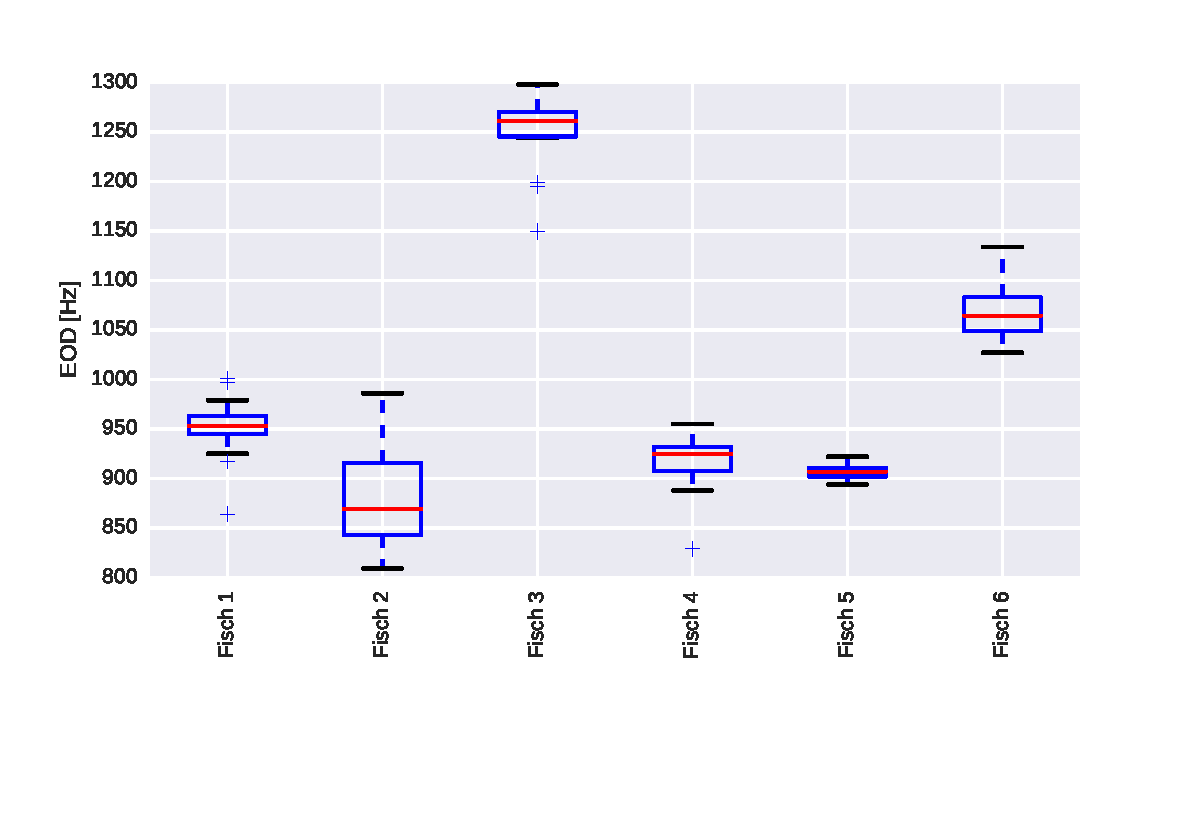
\includegraphics[height=8.5cm]{Abbildungen/eod_boxplot}
\caption{\label{fig:eods}Die EOD Frequenz Verteilung der Versuchstiere �ber den gesamten Versuchszeitraum gemessen. Die EOD Frequenz von Fisch 1 betrug im Median 955 Hz bei einem Quartilsabstand (IQR) von 15 Hz. Die EOD Frequenz von Fisch 2 hingegen war mit im Median 873 Hz etwas tiefer, bei einem IQR von 71 Hz. Fisch 3 hatte von allen Versuchstieren die h�chste EOD Frequenz und lag bei einem Median von 1261 Hz. Hier betrug der IQR 24,5 Hz. Der Median von Fisch 4 befand sich bei 927 Hz mit einem IQR von 12 Hz. 907 Hz betrug die mediane EOD Frequenz von Fisch 5 bei einem IQR von 9 Hz. Fisch 6 besa� mit einem Median von 1064.5 Hertz die zweit h�chste EOD Frequenz bei einem IQR von 34,25 Hz.}
\end{figure}

Wie in Abbildung \ref{fig:eods} zu sehen, variierten die EOD Frequenzen der Versuchstiere im Laufe des Versuchszeitraums. Wie beispielsweise von \citet{Enger1968} und \citet{Dunlap2000} beschrieben, beeinflusst die Wassertemperatur die EOD Frequenzen der Tiere. Demnach waren h�chstwahrscheinlich Schwankungen der Wassertemperaturen verantwortlich f�r die Schwankungen der EOD Frequenzen. 

\begin{figure}[H]
\centering
\subfigure[Fisch1]
{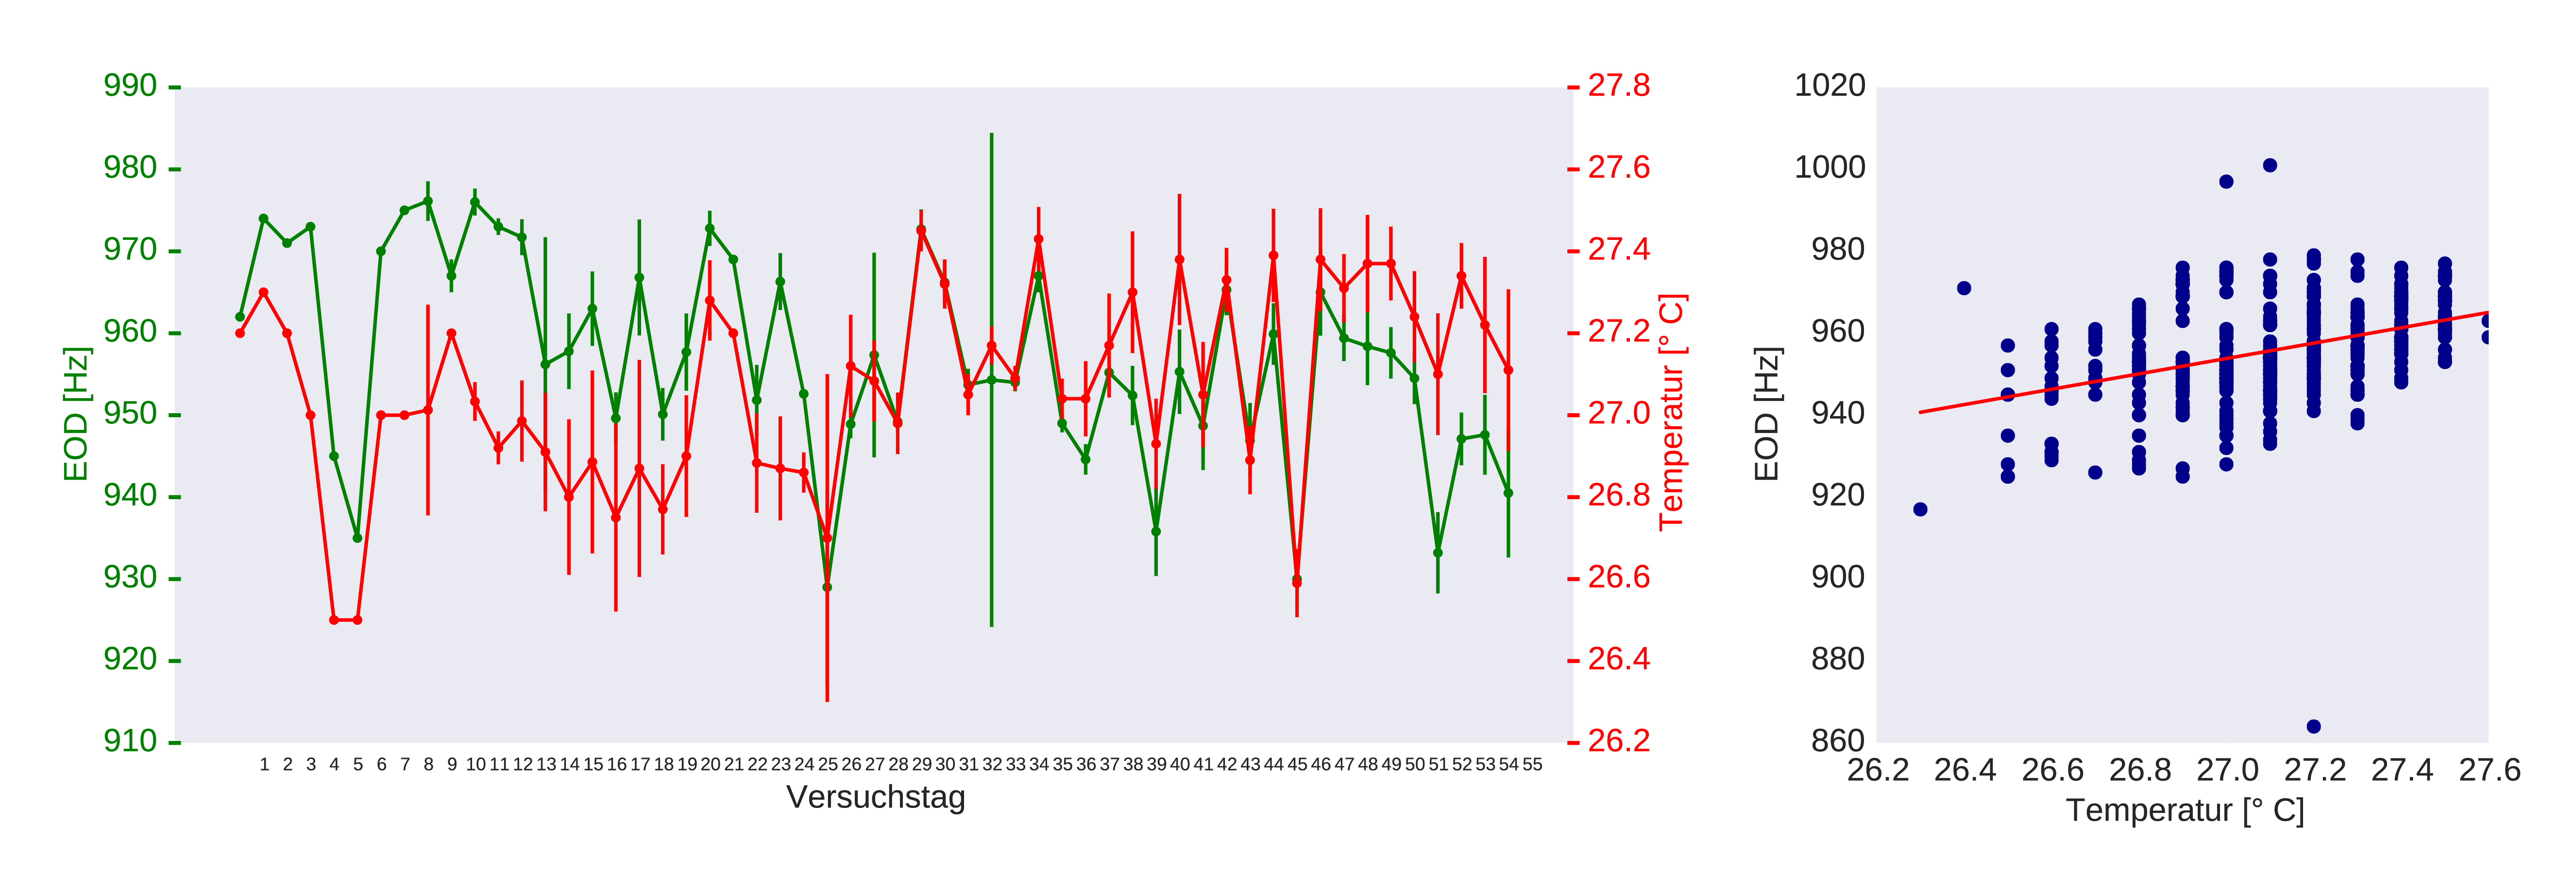
\includegraphics[height=5.5cm]{Abbildungen/temperatur1}}
\subfigure[Fisch2]
{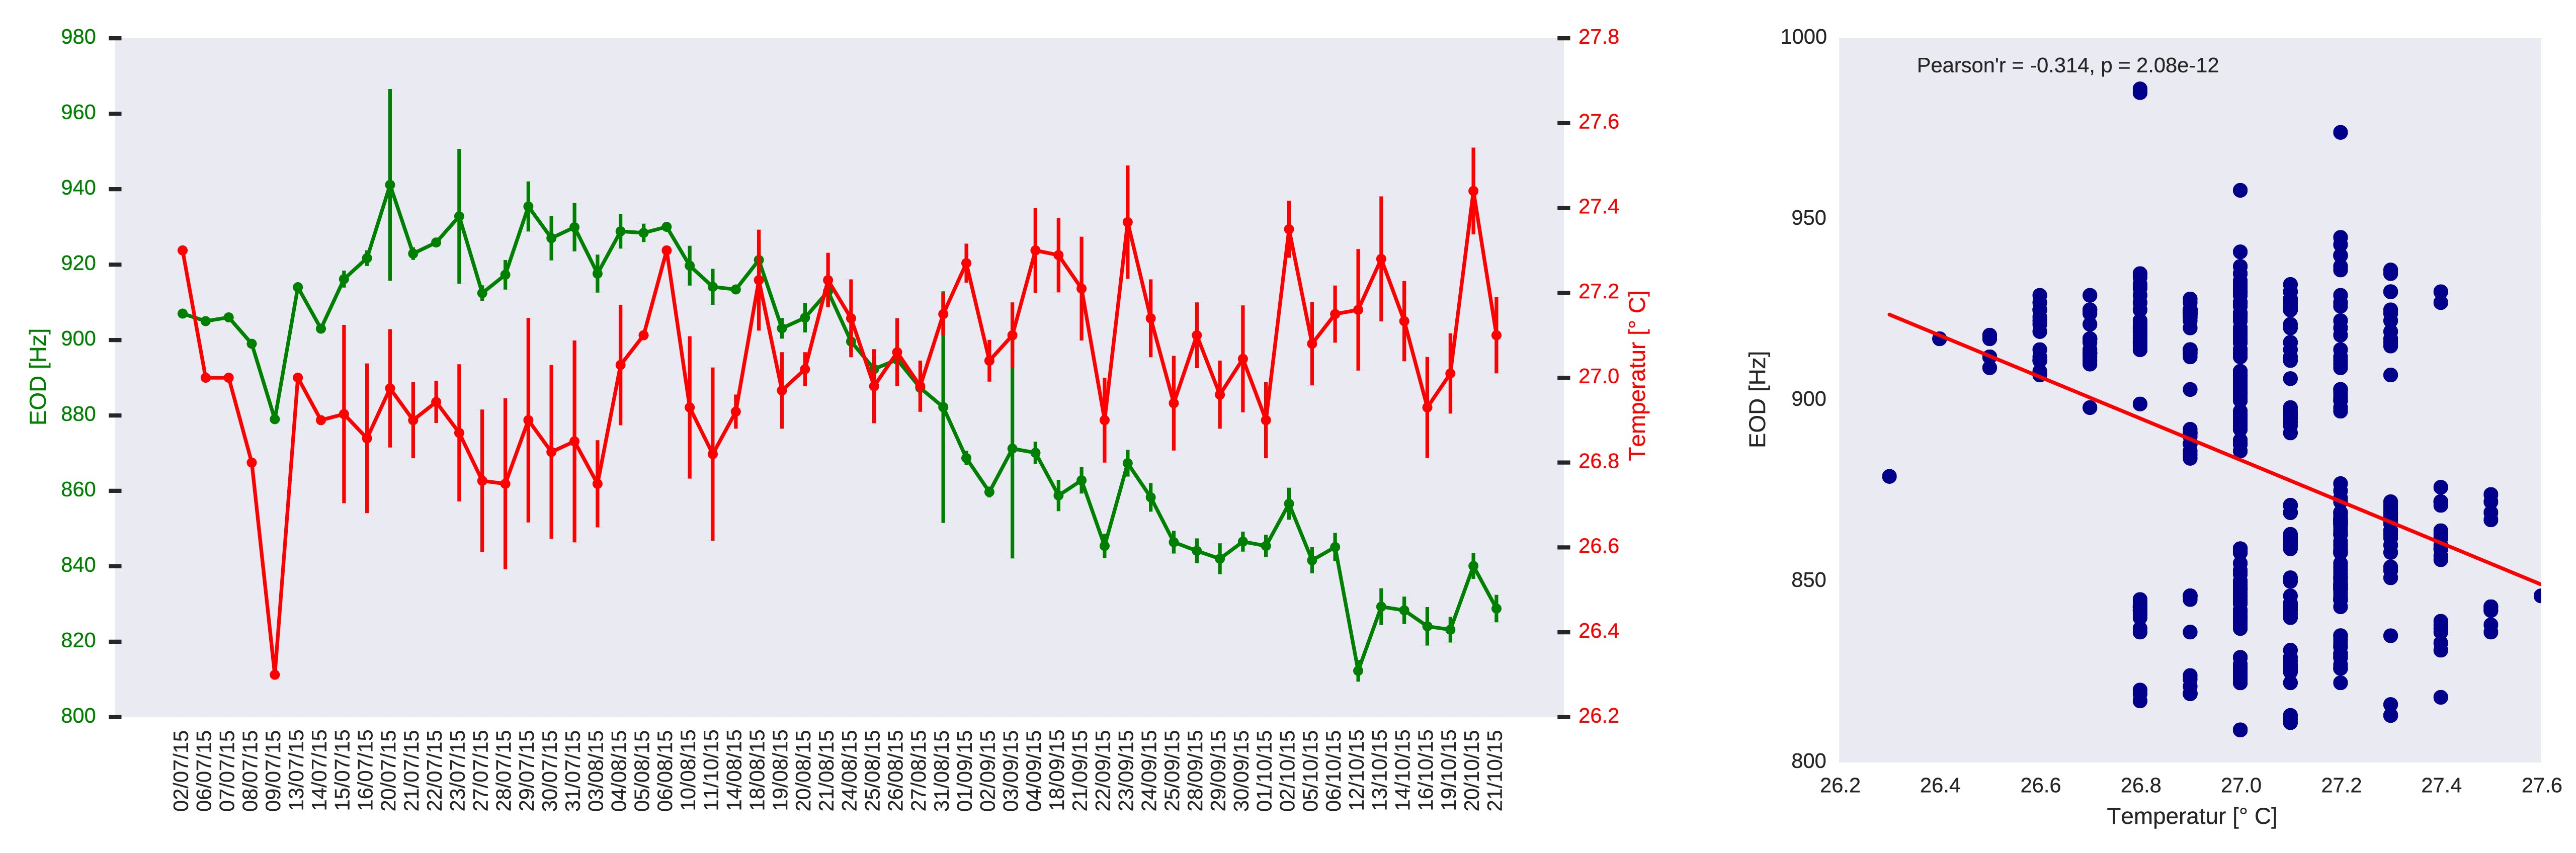
\includegraphics[height=5.5cm]{Abbildungen/temperatur2}}
\caption{\label{fig:temperatureod}Links: Die Graphik zeigt die Wassertemperaturen (rote Kurve) und die EOD Frequenzen von Fisch 1 (a) und Fisch 2 (b) in gr�n �ber die gesamte Versuchszeit einschlie�lich Vorversuche. Rechts: Korrelation der Wassertemperaturen und EOD Frequenzen. Als blaue Messpunkte sind die EOD Frequenzen mit zugeh�riger Wassertemperatur aller Versuchsdurchl�ufe dargestellt. In rot ist die daraus resultierende Regressionsgerade eingezeichnet.}
\end{figure}

Abbildung \ref{fig:temperatureod} zeigt hierbei den Einfluss der Temperatur auf die EOD Frequenzen von Fisch 1 (a) und Fisch 2 (b). Links ist f�r jedes der beiden Versuchstiere ein Graph mit zwei Y-Achsen zu sehen, welcher die mittlere EOD Frequenz (gr�n) und die mittlere Wassertemperatur (rot) jedes Versuchstags zeigt. Bei Fisch 1 ist hierbei eine Korrelation zwischen Wassertemperatur und EOD Frequenz zu beobachten: F�llt beispielsweise die mittlere Wassertemperatur von einem Versuchstag auf den n�chsten, so f�llt die EOD Frequenz gleicherma�en (siehe z.B Versuchstag 09/07/15). Rechts neben dem Graph ist ein zweiter Graph mit einer Regressionsgeraden zu sehen. Hier wurden die EOD Frequenzen und Wassertemperaturen jedes Versuchsdurchlaufs als Streudiagramm aufgetragen und eine Regressionsgerade daraus berechnet. Bei Fisch 1 betr�gt der Pearsons Korrelationskoeffizient 0,374 bei einem P-Wert von $1,6*10^{-15}$. Es liegt also eine lineare Korrelation von Temperatur und EOD Frequenz nahe. Allerdings geben \citet{Dunlap2000} f�r \emph{Apteronotus leptorynchus} $r^2$ Werte von �ber 0,97 an. Es w�re also eine st�rkere Korrelation von EOD Frequenz und Wassertemperatur zu erwarten gewesen. Bei Fisch 2 hingegen ist im linken Graphen mit der roten Temperaturkurve und der gr�nen EOD Frequenz Kurve keine lineare Korrelation zwischen EOD Frequenz und Wassertemperatur zu erkennen. Die EOD Frequenz von Fisch 2 scheint, von der Wassertemperatur unabh�ngig, im Laufe der Versuchstage abzunehmen. Die Regression ergibt au�erdem einen negativen Pearsons Korrelationskoeffizienten von -0,314 bei einem P-Wert von $2,08*10^{-12}$. Da eine lineare Korrelation von EOD Frequenzen und Wassertemperaturen bekannt ist \citep{Enger1968, Hopkins1976, Dunlap2000}, weichen die Ergebnisse von Fisch 2 stark von den Erwartungen ab. Zus�tzlich weist Fisch 2 eine weite Verteilung der EOD Frequenzen auf. So hat Fisch 2 bei der EOD Frequenzverteilung den h�chsten Quartilsabstand von 71 Hz (siehe Abb. \ref{fig:eods}). Aufgrund der gro�en Schwankungen der EOD Frequenz von Fisch 2 und der nicht vorhandenen Korrelation von EOD Frequenz und Wassertemperatur, k�nnte ein Messfehler beim Erfassen der EOD Frequenzen von Fisch 2 vorliegen. Dies h�tte starken Einfluss auf den Erfolg der Versuche, da die Stimuli ausgehend von der gemessenen EOD Frequenz generiert werden. Wurde die EOD Frequenz falsch bestimmt, so ist der Beat, welcher bei Interferenz der EOD Frequenz und der Stimuli entsteht, nicht konstant und das Versuchstier hat keinen Anhaltspunkt, anhand dessen es sich die Stimuli merken kann, da sie in diesem Fall willk�rlich in ihrer Frequenz variieren.

\begin{figure}[ht]
\centering
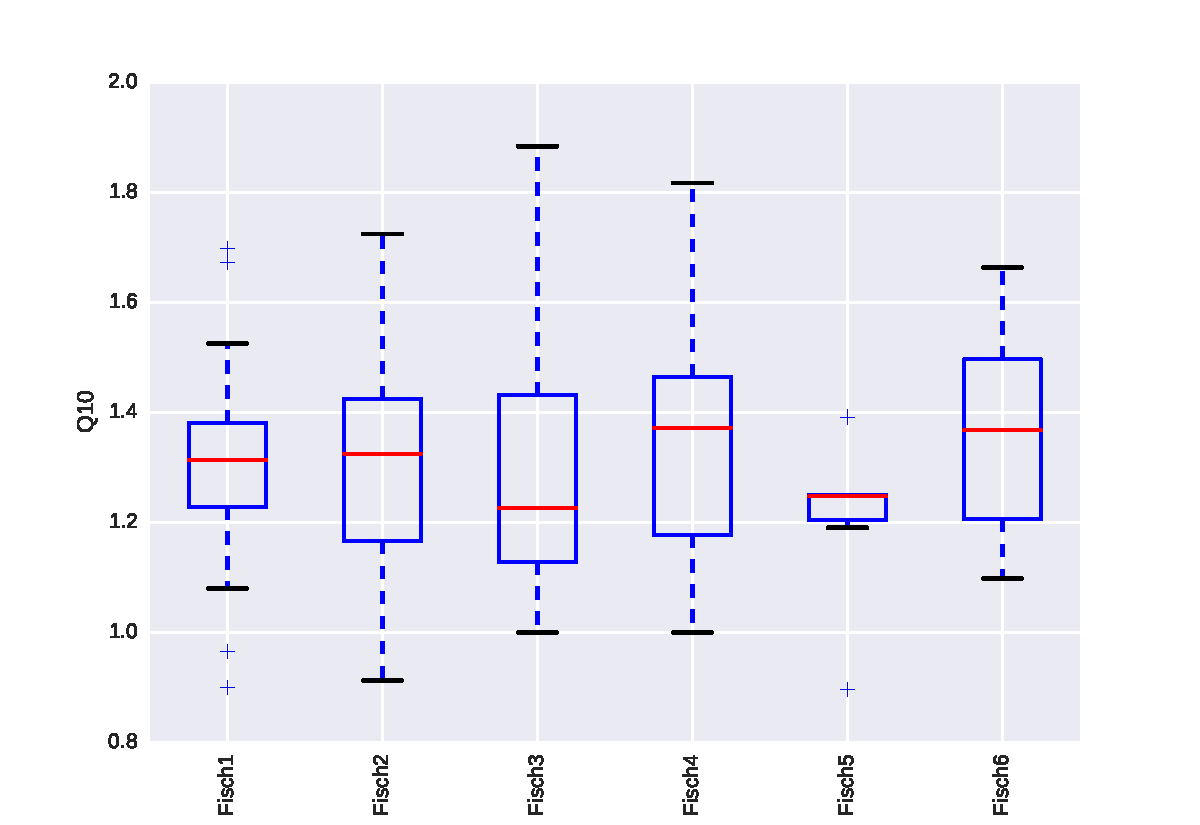
\includegraphics[height=7.5cm]{Abbildungen/q10_boxplot}
\caption{\label{fig:q10} Die Verteilung der $Q_{10}$-Werte aller Versuchstage f�r Fisch 1 - 6.}
\end{figure}

Zus�tzlich wurde f�r jedes der sechs Versuchstiere ein $Q_{10}$-Wert bestimmt. Dieser gibt an, um welchen Faktor die EOD Frequenz des Versuchstieres bei einem Anstieg der Wassertemperatur um 10 Kelvin ansteigt (siehe Tabelle \ref{fig:q10}). Hierbei ergab sich f�r alle Versuchstiere im Mittel ein $Q_{10}$-Wert von 1,3. In der Literatur werden f�r die Gattung \emph{Apteronotus} $Q_{10}$-Werte im Bereich von 1,5 \citep{Hopkins1976} bis 1,6 \citep{Dunlap2000} angegeben. Grund f�r die Abweichung k�nnte die eingeschr�nkte Messgenauigkeit des verwendeten Thermometers gewesen sein, welches lediglich eine Nachkommastelle angab.

\begin{table} [h] 
	\centering
	\caption{ Mediane $Q_{10}$-Werte aller Versuchstiere. Die Werte wurden wie folgt berechnet: Zun�chst wurde f�r jeden Versuchstag und jedes Versuchstier ein $Q_{10}$-Wert aus der maximalen (T2) und minimalen (T1) Wassertemperatur des Versuchstages und den dazugeh�rigen EODs (E1, E2) mit folgender Formel berechnet $Q_{10} = \frac{E2}{E1}^{ \frac{10}{T2-T1}}$. Anschlie�end wurde der Median aus den $Q_{10}$-Werten aller Versuchstage berechnet.}
	\vspace{0,2cm}	
	\begin{tabular}{cccc} %eigentliche Tabelle 
		\toprule % d�nne Linie 
			& $Q_{10}$-Wert \\
		 Fisch 1 (2015albi02):& 1,31 \\
		 Fisch 2 (2015albi01):& 1,33 \\
		 Fisch 3 (2014albi08):& 1,23 \\
		 Fisch 4 (2013albi14):& 1,37 \\
		 Fisch 5 (2013albi09):& 1,25 \\
		 Fisch 6 (2012albi01):& 1,37 \\
		\bottomrule % bi�chen dickere Linie unten
	\end{tabular}
	\label{q10}
\end{table}

Wie in Abbildung \ref{fig:conductivity} am Beispiel von Fisch 1 dargestellt, hatte die Leitf�higkeit des Wassers keinen Einfluss auf die EOD Frequenz der Versuchstiere. So liegt der Korrelationskoeffizient von Pearson bei -0,055 bei einem P-Wert von 0,26. Es liegt also keine Korrelation von EOD Frequenz und Leitf�higkeit vor.

\begin{figure}[ht]
\centering
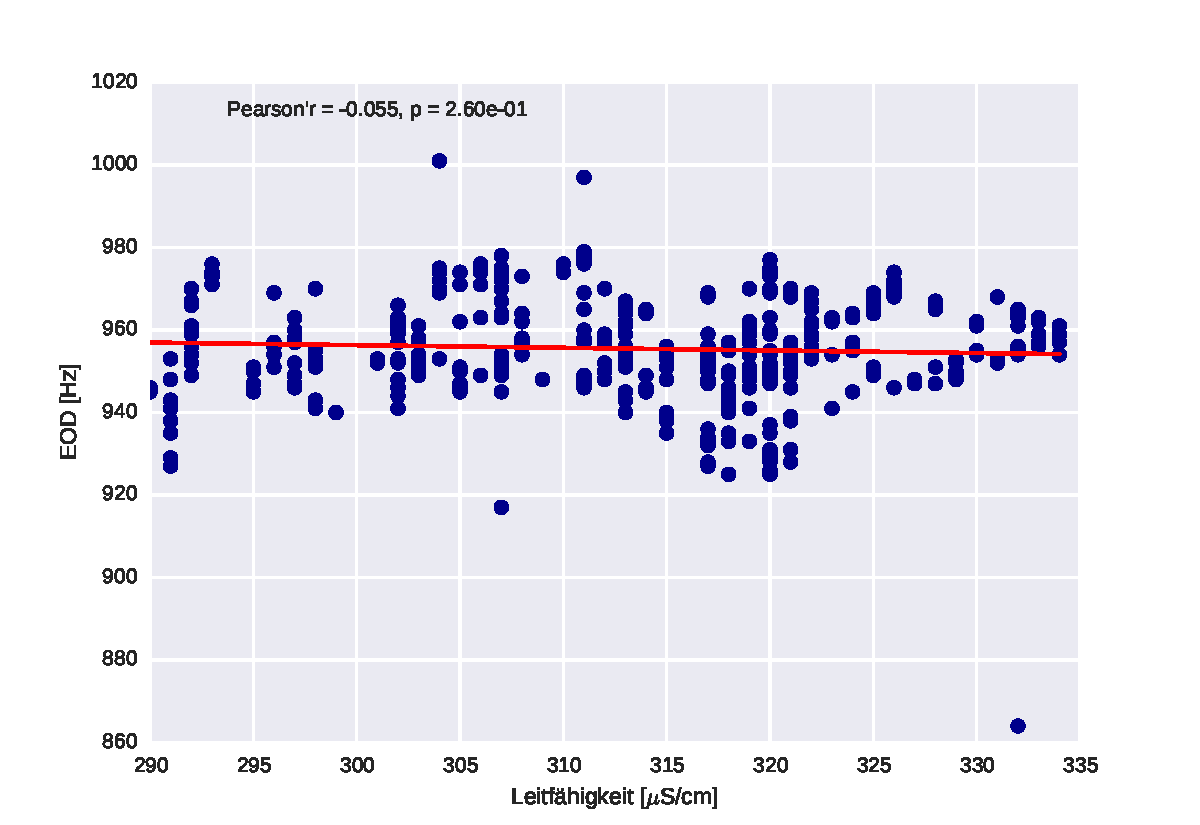
\includegraphics[height=7.5cm]{Abbildungen/conductivity}
\caption{\label{fig:conductivity}Korrelation von Leitf�higkeit und EOD Frequenz bei Fisch 1. In blau sind in einem Streudiagramm alle Messwerte aller Versuchsdurchl�ufe eingetragen. In rot ist die daraus berechnete Regressionsgerade eingezeichnet.}
\end{figure}

\section{Lernerfolg der Versuchstiere}

Fisch 1 und Fisch 2 gingen nach 9 Versuchstagen von der ersten Phase, der \emph{Eingew�hnung}, in die n�chste Phase, die \emph{Konditionierung auf S+}, �ber. Da Fisch 3 und Fisch 4 schlechter kooperierten, gingen diese erst nach elf Versuchstagen in die n�chste Phase �ber. Wie in Abbildung \ref{fig: versuch1_zeit} im Ergebnisteil aufgezeigt wurde, verringerte sich die mittlere Zeit, welche Fisch 1 und Fisch 2 ben�tigten, um einen Versuchsdurchlauf in der Eingew�hnung erfolgreich abzuschlie�en, mit der Anzahl der bereits absolvierten Versuchstage. Daraus l�sst sich schlie�en, dass Fisch 1 und Fisch 2 lernten, dass an den Elekrtroden Futter zu finden war. Bei Fisch 3 und Fisch 4 hingegen schwankten die mittleren Zeiten stark. Bei beiden Tieren ist eine Art Zickzackmuster im Verlauf der mittleren Zeitkurve erkennbar. Besonders bei Fisch 4 ist auff�llig, dass auf einen Versuchstag, an dem er eine kurze mittlere Versuchsdurchlaufzeit hatte, ein Tag folgte, an welchem er schlecht kooperierte und die mittleren Versuchszeiten lang waren. Eine m�gliche Erkl�rung f�r dieses Verhalten w�re, dass die beiden Versuchstiere (Fisch 3 und 4) nach einem erfolgreichen Versuchstag, an welchem wegen k�rzerer Versuchszeiten mehr Versuchsdurchl�ufe stattfinden konnten und somit auch mehr Larven verf�ttert wurden, am n�chsten Tag keinen Hunger mehr hatten. Dagegen spricht allerdings, dass es sich bei den Tagen, an welchen die Fische schlecht abschnitten, h�ufig um Montage handelte und zu erwarten gewesen w�re, dass die Tiere nach dem Wochenende hungrig sind. Au�erdem handelte es sich bei den unstet abschneidenden Versuchstieren Fisch 3 und Fisch 4 um die ausgewachsenen adulten Tiere, die etwa die doppelte K�rperl�nge der juvenilen Tieren (Fisch 1 und 2) ma�en. Daher ist die Annahme, Fisch 3 und 4 seien nicht hungrig gewesen, w�hrend die juvenilen Tiere es aber waren, unwahrscheinlich. 
Eine wahrscheinlichere Erkl�rung f�r das schnellere Lernen und das bessere Abschneiden von Fisch 1 und 2 k�nnte sein, dass die Versuche wenige Tage nach der Lieferung der Jungtiere gestartet wurden und diese an noch keinen F�tterungsablauf in der neuen Umgebung gew�hnt waren, weswegen sie m�glicherweise noch lernf�higer waren als die adulten Tiere, welche bereits seit etwa einem (Fisch 3) oder sogar zwei (Fisch 4) Jahren an eine F�tterung in ihrem Tank gew�hnt waren.
Was sich bereits im ersten Vorversuch gezeigt hatte, zog sich durch die weiteren Vorversuche und den Hauptversuch durch. So schnitten, wie in Abbildung \ref{fig: erfolgsquote} zu sehen, Fisch 1 und Fisch 2 auch bei den beiden weiteren Vorversuchen besser ab und konnten wegen geringerer Zeiten, welche f�r einen Versuchsdurchlauf ben�tigt wurden, auch insgesamt mehr Versuchsdurchl�ufe pro Vorversuch absolvieren. Fisch 3 wurde aufgrund der Teilnahmeverweigerung am letzten Vorversuch, an welchem er die Startbox kaum freiwillig verlie�, vom Hauptversuch ausgeschlossen.

Im Hauptversuch wurden au�erdem noch die beiden Versuchstiere Fisch 5 und Fisch 6 dazugenommen, welche den Versuch bereits im Rahmen einer vorangegangenen Bachelorarbeit neun Monate zuvor erlernt hatten. Als S+ und S- Stimulus waren f�r beide Versuchstiere dieselben Beatfrequenzen gew�hlt worden, auf welche die Fische in der vorangegangenen Arbeit trainiert worden waren. Beide Versuchstiere schienen sich aber nicht mehr an den Versuchsablauf zu erinnern. So verlie� Fisch 5 kaum einmal die Startbox. Fisch 6 kooperierte zwar besser und verlie� die Startbox, w�hlte aber keine der beiden Elektroden aus.  Die Versuchstiere erinnerten sich auch nach mehreren Versuchstagen nicht an den Ablauf der Versuche.  Eine m�gliche Erkl�rung daf�r w�re, dass die Fische in der Zwischenzeit an anderen Verhaltensexperimenten teilgenommen hatten und dadurch das alte Experiment vergessen wurde. Diese Erkl�rung ist allerdings nur f�r Fisch 6 schl�ssig, da Fisch 5 in der Zwischenzeit an keinen anderen Versuchen teilgenommen hatte. Vermutlich lag jedoch der Grund darin, dass der versuchsfreie Zeitraum von neun Monaten schlicht zu lang war. So wurde beispielsweise bei dem schwach elektrischen Fisch \emph{Apteronotus leptorhynchus} gezeigt, dass dieser Artgenossen anhand ihrer EOD Frequenz identifizieren kann. Die Erinnerung an diese Frequenz verschwand aber nach einigen Tagen \citep{Harvey-Girard2010}. �hnliches w�re daher vermutlich auch bei \emph{Apteronotus albifrons} bez�glich ihres Erinnerungsverm�gens an die Beatfrequenzen zu erwarten.

Auch anhand der Positionen, welche die Fische im Versuchsbecken h�ufig frequentierten (siehe Abb.\ref{fig: heatmap_positions}), und anhand der Geschwindigkeiten an den Elektroden und entfernt von den Elektroden (siehe Abb. \ref{fig: boxplot_geschwindigkeit}) ist der Lernerfolg der Versuchstiere erkennbar. So verlangsamten Fisch 1 und 2 ihre Schwimmgeschwindigkeit signifikant, wenn sie sich in der N�he der Elektroden befanden. Fisch 4 und Fisch 6 hingegen waren sogar im Bereich der Elektroden sigifikant schneller als abseits der Elektroden. Sie hatten also nicht erlernt, dass sie eine der beiden Elektroden ausw�hlen sollten. Entsprechendes ergab die Analyse der Positionen, an welchen sich die Versuchstiere aufhielten (siehe Abb. \ref{fig: heatmap_positions}). So hielten sich Fisch 1 und Fisch 2 h�ufig im Bereich der Elektroden auf, w�hrend Fisch 4 und Fisch 6 keine besondere Pr�ferenz f�r den Bereich um die Elektroden herum zeigten, sondern sich lediglich h�ufiger am Beckenrand aufhielten, was vermutlich damit zusammenh�ngt, dass die Tiere offene Fl�chen meiden.
 
Es war zu erwarten, das es f�r \emph{Apteronotus albifrons} m�glich ist, die Aufgabe zu erlernen, eine Elektrode auszuw�hlen. So wurde bereits in anderen Konditionierungsversuchen gezeigt, dass schwach elektrische Fische beispielsweise darauf trainiert werden k�nnen, Objekte anhand der Gr��e, Form oder anhand des Materials zu unterscheiden und auszuw�hlen \citep{Emde2007}. Auch wurde \emph{Apteronotus albifrons} bereits von \citet{Knudsen1974} darauf konditioniert, eine Stimuluselektrode, welche eine Sinusschwingung verschiedener Frequenzen abgab, von einer Stimuluselektrode zu diskriminieren, welche kein Signal abgab \citep{Knudsen1974}. Dennoch scheint die in dieser Arbeit gestellte Aufgabe f�r die Tiere eine komplexe und schwierige Aufgabe zu sein. So erlernten lediglich zwei von vier Versuchstieren die Aufgabe. Auch die beiden Versuchstiere Fisch 5 und 6, welche erst beim Hauptversuch hinzugezogen wurden und die Aufgabe zuvor schon einmal erlernt hatten, waren nicht dazu in der Lage, die Aufgabe innerhalb der Hauptversuchszeit erneut zu erlernen.

\section{Objektivit�t der Daten}

Bei einem Experiment, bei welchem die versuchsduchf�hrende Person wei�, welche Elektrode, die belohnte und welche die unbelohnte ist, kann es zu einer unbewussten Beeinflussung des Versuchs und einer Verschiebung der Daten in die gew�nschte Richtung kommen. Um zu �berpr�fen, wie objektiv entschieden wurde, ob das Versuchstier eine Elektrode ausw�hlte, wurden mit Hilfe der Videoaufnahmen zwei wichtige Parameter zur Bewertung, ob eine Elektrode ausgew�hlt wurde, betrachtet. Dabei wurden die Parameter auf Unterschiede hin untersucht, wenn die belohnte Elektrode und wenn die unbelohnte Elektrode ausgew�hlt wurde. 

\subsubsection{Distanz zu den Stimuluselektroden}

\begin{figure}[ht]
\centering
{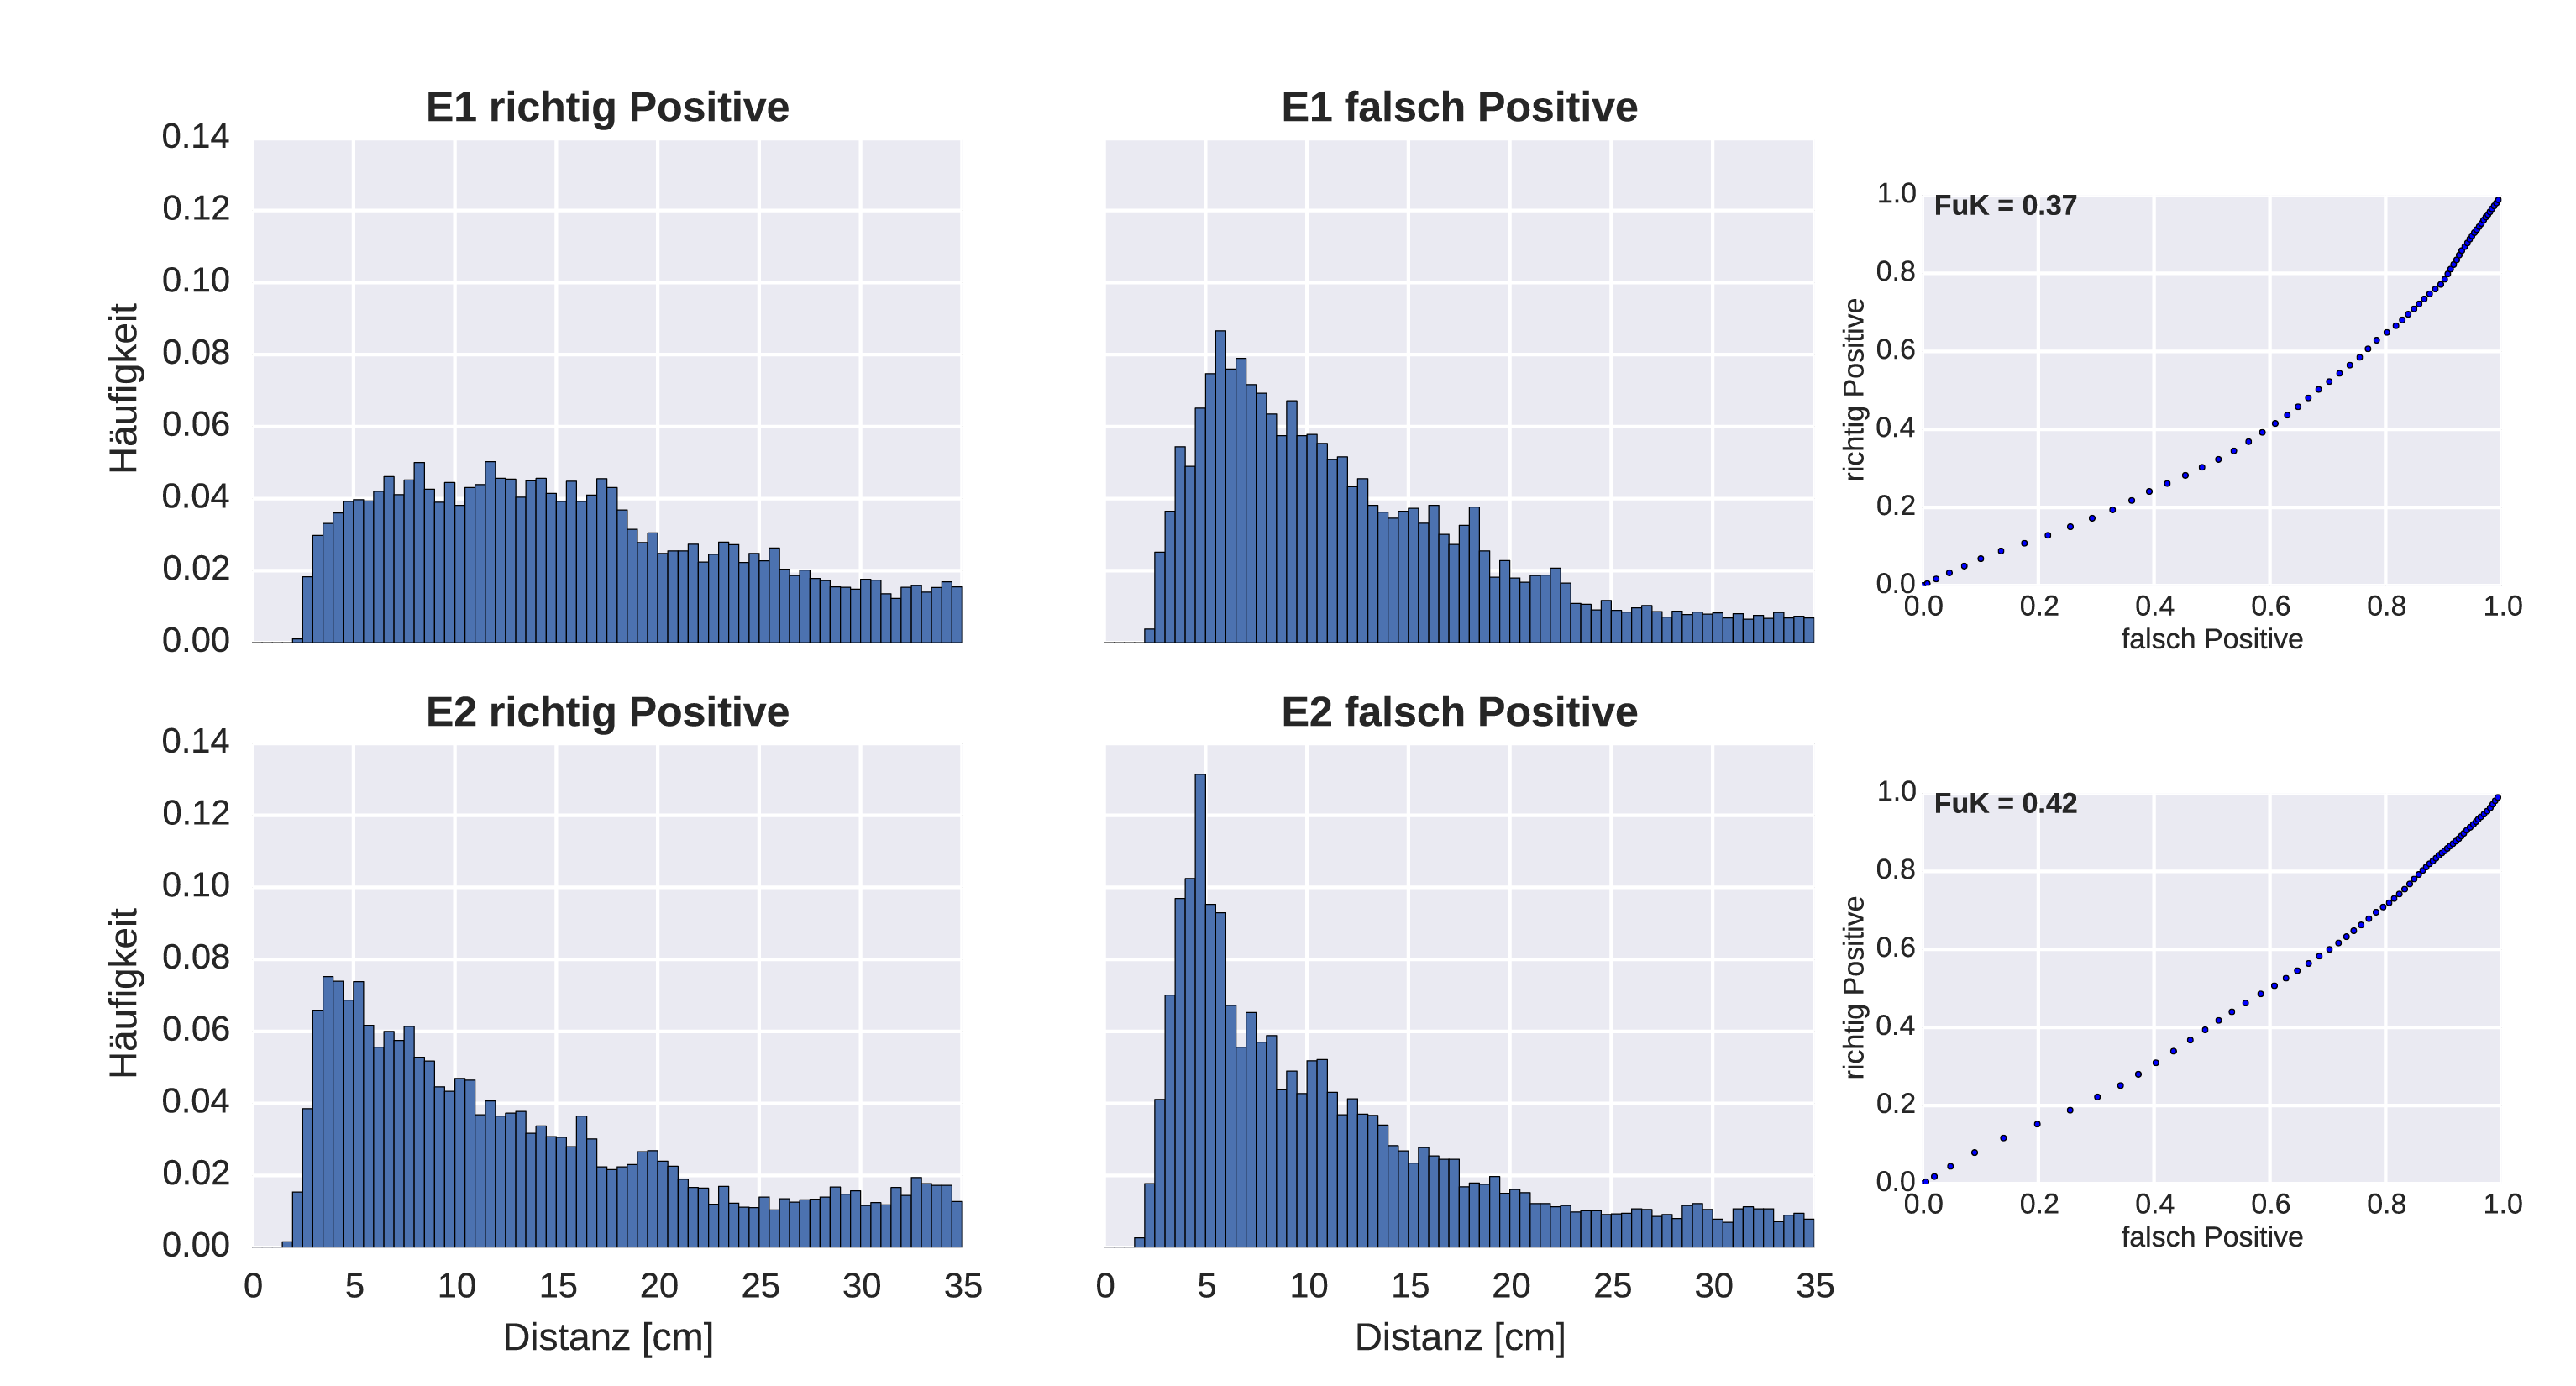
\includegraphics[height=8.5cm]{Abbildungen/Histogramm_Elektrodendistanzen_mit_Fischentscheidung2015albi02}}
\caption{\label{fig:distanzen_entscheidung} Fisch 1 Distanzen Histogramme. Links oben: Histogramme f�r Elektrode 1. Auf der X-Achse ist die Distanz zur jeweils ausgew�hlten Elektrode aufgetragen. Auf der Y-Achse ist die H�ufigkeit der Distanz aufgetragen. Rechts oben: ROC Kurve von Elektrode 1. Links unten: Histogramme Elektrode 2. Recht unten: ROC Kurve von Elektrode 2.}
\end{figure}

Abbildung \ref{fig:distanzen_entscheidung} zeigt beispielhaft das Vorgehen f�r Fisch 1. Hierbei wurde �berpr�ft, welche Distanzen zu einer Elektrode bestanden, wenn sie ausgew�hlt wurde. In den vier Histogrammen ( siehe Abb. \ref{fig:distanzen_entscheidung}) wurden f�r Elektrode 1 und Elektrode 2 je die Verteilungen der Distanzen zu einer Elektrode, wenn die Elektrode den belohnten Stimulus abgab und ausgew�hlt wurde (richtig Positive) und zu der Elektrode, wenn sie den unbelohnten Stimulus abgab und ausgew�hlt wurde (falsch Positive), aufgetragen.  
Rechts neben den richtig positiven und falsch positiven Histogrammen f�r Elektrode 1 und Elektrode 2 ist jeweils eine sogenannte ROC Kurve abgebildet. Bei der Receiver Operating Characteristic (ROC) handelt es sich um eine Technik, mit welcher Analysestrategien bewerten werden k�nnen \citep{Fawcett2004}.
Auf der X-Achse der ROC Graphen ist jeweils die falsch-positiv-Rate dargestellt, w�hrend auf der Y-Achse die richtig-positiv-Rate aufgetragen ist. Die Abk�rzung FuK steht f�r "Fl�che unter der Kurve".  Bei Elektrode 1 betr�gt die FuK 0,37, w�hrend sie bei Elektrode 2 0,42 betr�gt. L�ge der Wert bei 0,5, dann w�ren die Distanzen zu den Elektroden, unabh�ngig davon, ob die Elektrode den belohnten Reiz abgab oder den unbelohnten, gleich. Dass die Fl�chen etwas unter 0,5 liegen, weist darauf hin, dass es etwas h�ufiger zu geringen Elektrodendistanzen kam, wenn die Elektrode den unbelohnten Reiz abgab. Gleiches ergab sich f�r Fisch 2, bei welchem sich Werte f�r die FuK von 0,35 bei Elektrode 1 und 0,41 bei Elektrode 2 ergaben.
Eine m�gliche Erkl�rung daf�r, dass die Versuchstiere etwas h�ufiger niedrige Distanzen zu den Elektroden hatten, wenn diese den unbelohnten Stimulus abgaben, k�nnte in der Versuchsdurchf�hrung liegen: Wenn das Versuchstier die belohnte Elektrode ausw�hlte, wurde die Videoaufnahme gestoppt, der Stimulus aber angelassen und der Fisch musste noch einige Zeit an der Elektrode verweilen, bis er ein Feedback in Form der Belohnung bekam. Der Fisch verweilte in diesem Fall also noch einige Zeit von den Videoaufnahmen unerfasst in kurzer Distanz zu den Elektroden. Wenn das Versuchstier aber die unbelohnte Elektrode ausw�hlte, kam es direkt zu einem Feedback, da der Stimulus direkt zeitgleich mit dem Video ausgeschaltet wurde. Um die Zeit bis zu einem Feedback ungef�hr gleich lang zu gestalten, wurde daher bei der Auswahl eines unbelohnten Stimulus etwas l�nger damit gewartet, die Videoaufnahme zu stoppen, als bei der Auswahl eines belohnten Stimulus, wodurch das Versuchstier bei einem unbelohnten Stimulus in der Videoaufnahme immer etwas l�nger in kurzer Distanz zur Elektrode verweilte. Dies k�nnte erkl�ren, weshalb die FuKs etwas unter 0,5 lagen. 

\subsubsection{Schwimmgeschwindigkeit an den Stimuluselektrode}

\begin{figure}[ht]
\centering
{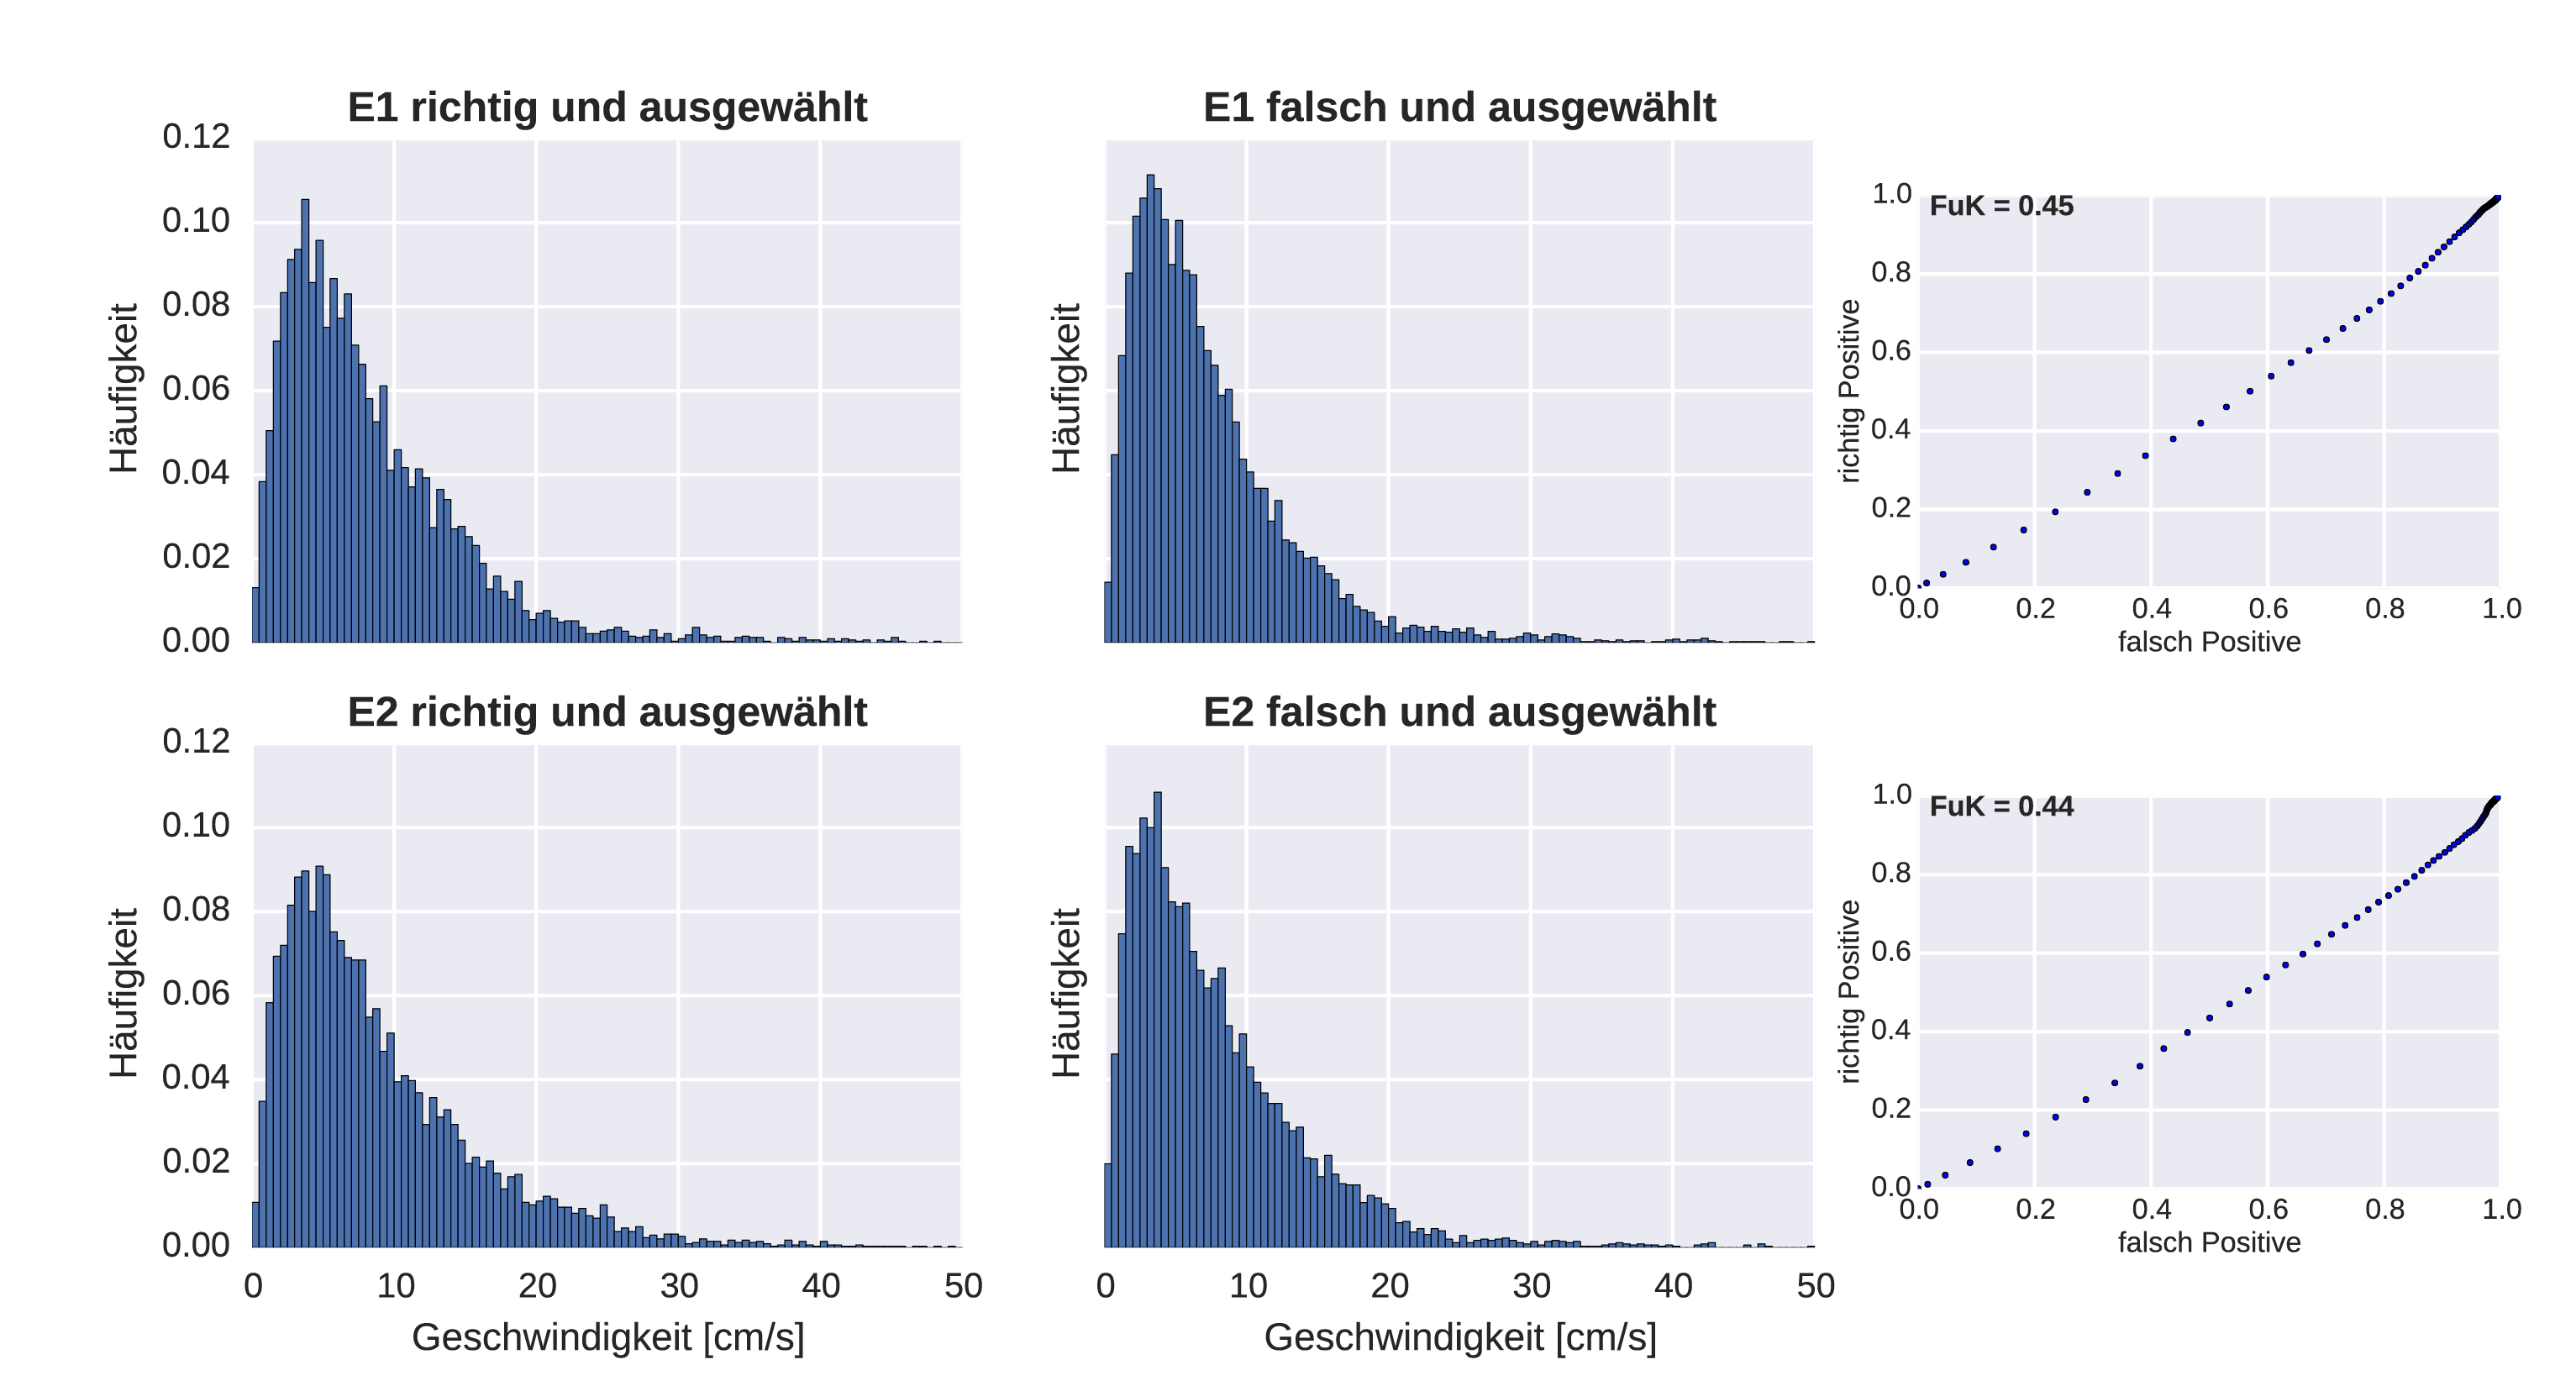
\includegraphics[height=8.5cm]{Abbildungen/Histogramm_Geschwindigkeiten_mit_Fischentscheidung2015albi02}}
\caption{\label{fig:geschwindigkeiten_entscheidung}Fisch 1 Geschwindigkeitshistogramme. Links oben: Histogramme f�r Elektrode 1. Hier ist die Geschwindigkeit in der N�he der Elektroden (Distanz $<$ 12 cm) gegen die H�ufigkeit, mit welcher sie vorkam, aufgetragen. Rechts oben: ROC Kurve von Elektrode 1. Links unten: Histogramme Elektrode 2. Recht unten: ROC Kurve von Elektrode 2.}
\end{figure}

Analog zum Vorgehen bei den Elektrodendistanzen wurden auch die Schwimmgeschwindigkeiten an den Elektroden verglichen, wenn die Elektrode mit dem belohnten Stimulus (S+) ausgew�hlt wurde und wenn die Elektrode mit dem unbelohnten Stimulus (S-) ausgew�hlt wurde.
Abbildung \ref{fig:geschwindigkeiten_entscheidung} zeigt dazu die Histogramme f�r Fisch 1. Wie in der Abbildung zu sehen ist, unterscheiden sich die einzelnen Histogramme kaum voneinander. Auch die ROC Kurven f�r Elektrode 1 und Elektrode 2 rechts neben den Histogrammen fallen dementsprechend aus: Mit einer FuK von 0,45 bzw. 0,44 zeigen beide ROC Kurven, dass die Schwimmgeschwindigkeiten unabh�ngig davon, ob die Elektrode mit einem belohnten Reiz oder mit einem unbelohnten Reiz ausgew�hlt wurde, gleicherma�en gesenkt wurde. Gleiches galt f�r Fisch 2, dessen FuK bei Elektrode 1 bei 0,41 und bei Elektrode 2 bei 0,45 lag.

Da keine wesentlichen Unterschiede in der Schwimmgeschwindigkeit an den Elektroden und in der Distanz zu den Elektroden bei einer Auswahl der belohnten und der unbelohnten Elektrode bestand, scheint eine unbewusste Beeinflussung der Daten eher gering gewesen zu sein . Auch andere Beeinflussungen der Versuchstiere von au�en beispielsweise durch K�rpersprache des Versuchsdurchf�hrenden sind unwahrscheinlich, da die versuchsdurchf�hrende Person mit dem R�cken zum Versuchsbecken sa� und das Versuchsbecken abgeklebt war. Dennoch w�re es bei nachfolgenden Experimenten sinnvoll, den Versuch zu einem doppelblinden Experiment zu machen, bei welchem die versuchsdurchf�hrende Person erst, nachdem der Fisch eine der Elektroden ausgew�hlt hat, die Information bekommt, ob es sich um die belohnte oder die unbelohnte Elektrode handelte. 

\section{K�nnen die Versuchstiere die Stimuli unterscheiden?}

Da nur Fisch 1 und Fisch 2 den Ablauf des Hauptversuchs erlernten, konnte der Konditionierungserfolg nur bei diesen Versuchstiere bemessen werden. Hierbei konnte gezeigt werden, dass eines der beiden Versuchstiere (Fisch 1) signifikant h�ufiger die Elektrode mit dem belohnten Stimulus ausw�hlte. Allerdings w�hlte das Versuchstier im Median nur in Rund 60 Prozent der F�lle die belohnte Elektrode aus, was nicht hinreichend zeigt, dass das Versuchstier die Stimuli unterscheiden konnte. Das zweite Versuchstier (Fisch 2) zeigte zun�chst eine Pr�ferenz zu dem eigenmanniaartigen Stimulus. Diese erwies sich jedoch bei weiteren Tests als nicht signifikant. Insgesamt schien sich das Tier zuf�llig f�r einen der Stimuli zu entscheiden, ungeachtet dessen, ob dieser belohnt oder unbelohnt war. Daher bleibt, offen, ob \emph{Apteronotus albifrons} die in den P-Units und in den Pyramidenzellen des ELL vorhandenen Informationen �ber weit au�erhalb des eigenen EOD Frequenzbereichs liegende Frequenzen verarbeiten und aktiv nutzen kann. Dennoch weisen zahlreiche Studien daurauf hin, dass dies \emph{Apteronotus albifrons} m�glich sein sollte . So testete \citet{Knudsen1974} bereits, auf welche Frequenzen \emph{Apteronotus albifrons} eine Verhaltensreaktion zeigte. Dabei fand er heraus, dass \emph{Apteronotus albifrons} Verhaltensreaktionen auf sinusf�rmige elektrische Feldern zwischen 5 und 3000 Hz zeigte. Dies war allerdings nur bei einer sehr hohen Feldintensit�t (1mV/cm) der Fall. Bei niedrigeren Intensit�ten (10-20 $\mu$V/cm) konnten nur Frequenzen von 700-1300 Hz, welche etwa der EOD Frequenz von Artgenossen entsprechen, eine Verhaltensreaktion hervorrufen. M�glicherweise war daher die Stimulusamplitude, welche in dem Experiment dieser Arbeit gew�hlt wurde, zu gering, weshlab \emph{Apteronotus albifrons} gegebenenfalls den niedrigen Frequenzanteil des eigenmanniaartigen Signals nicht oder nur schwer wahrnehmen konnte. Die Feldintensit�t betrug im Versuchsbecken mittig zwischen den Stimuluselektroden knapp 0,3 mV (siehe Tabelle \ref{fig:amplitude2}). Zwar wurde die Stimulusamplitude im Laufe des Hauptversuchs verdoppelt ohne, dass es zu einer signifikanten Verhaltens�nderung der Versuchstiere kam, m�glicherweise reichte diese Erh�hung jedoch nicht aus. Die gew�hlte Stimulusamplitude entsprach in etwa der Intensit�t, bei welcher die Tiere elektrische Signale mit einer Frequenz nahe der eigenen EOD Frequenz wahrnehmen k�nnen \citep{Fotowat2013}. Die f�r den reinen Sinusstimulus ausgew�hlten Frequenzen, welche im Bereich $\pm100$ Hz Differenz von der EOD Frequenz lagen, m�ssten f�r die Versuchstiere demnach optimal wahrnehmbar gewesen sein, zumal die P-Units bei Beatfrequenzen zwischen 20 und 130 Hz am empfindlichsten sind\citep{Walz2014}. Es liegt also nahe, dass \emph{Apteronotus albifrons} zwar in der Lage dazu ist, Frequenzen weit au�erhalb der eigenen EOD Frequenz wahrzunehmen, allerdings nur bei einer entsprechend hohen Signalintensit�t. Diese Hypothese wird ebenfalls durch die noch unver�ffentlichte Arbeit von \citet{Henninger2015} gest�tzt, welcher das Balzverhalten von \emph{Apteronotus leptorynchus} beobachtete. Dabei war auff�llig, dass zwei Fische unterschiedlichen Geschlechts r�umlich nahe beieinander waren, da hier wegen der weit auseinanderliegenden EOD Frequenzen, sehr hohe Beatfrequenzen entstanden. Um diese wahrzunehemen  r�umlich sehr nah beieinander befanden. Die Kommunikation zwischen rivalisierenden M�nnchen hingegen erfolgt auch �ber sehr gro�e Distanzen. Hierbei handelt es sich um niedrige Beatfrequenzen, da die EOD Frequenzen der beiden gleichgeschlechtlichen Tiere nahe beieinander liegen. Bei hohen Beatfrequenzen scheint im Gegensatz zu niedrigen Beatfrequenzen eine gro�e r�umliche N�he notwendig zu sein, wodurch das Signal des einen Kommunikationspartners bei dem anderen Individuum mit einer hohen Intensit�t ankommt, welche offenbar notwendig zur Wahrnehmung der Frequenz ist.

Abschlie�end l�sst sich daher festhalten, dass in diesem Experiment zwar nicht gezeigt werden konnte, dass \emph{Apteronotus albifrons} dazu in der Lage ist, Signale weit au�erhalb der arteigenen EOD Frequenz wahrzunehmen, dies aber trotzdem sehr wahrscheinlich ist. Bei nachfolgenden Experimenten sollte eine h�here Stimulusamplitude gew�hlt werden, so dass die Feldintensit�t bei etwa 1mV/cm liegt. Dar�ber hinaus k�nnten starke Schwankungen der EOD Frequenz, welche eine st�ndige �nderung der der Stimulusfrequenzen bewirken, wie es beispielsweise bei Fisch 2 der Fall war, den Fisch irritieren. Daher sollte wegen der Korrelation zwischen EOD Frequenz und Wassertemperatur die Wassertemperatur m�glichst noch konstanter gehalten werden. Des Weiteren w�re f�r nachfolgende Experimente eine doppelblindes Vorgehen, bei welchem auch der versuchsdurchf�hrenden Person nicht bekannt ist, welche Elektrode den unbelohnten Reiz abgibt, ratsam.






\thispagestyle{empty}

\noindent Die vorliegende Arbeit wurde unter Leitung von Herrn Prof. Dr. Benda im Zeitraum Juni 2015 bis Dezember 2015 in der Abteilung Neuroethologie am Institut f�r Neurobiologie der Eberhard Karls Universit�t T�bingen angefertigt.


\vspace{5cm}


\textbf{\Huge Danksagung}

\vspace{1cm}

Diese Arbeit w�re nicht ohne die gro�e Unterst�tzung und die zahlreichen Anregungen und Hilfestellung von verschiedensten Seiten entstanden. Daf�r m�chte ich mich bei allen beteiligten Personen bedanken.
 
An erster Stelle m�chte ich mich hierf�r bei Doktor Jan Grewe f�r die Bereitstellungen des spannenden und interessanten Themas, als auch f�r die exzellente Betreuung und die zahlreichen Diskussionen bedanken.

Au�erdem m�chte ich dem gesamten Arbeitskreis - blabalabala, blublubblub f�r das angenehme Arbeitsklima und die zahlreichen Anregungen danken. Vielen Dank, dass ihr ein produktives Arbeiten m�glich gemacht habt. 


\bibliographystyle{standard}
\bibliography{Literatur}

%%\include{Anhang}
%
\end {document}
%
%
%
%
%
%%n�tzliche befehle: \FloatBarrier -> vll hilft es die tabellen gescheit zu setzen
%% \textsc{Nicholson} f�r namen